\documentclass[12pt,a4paper]{report}

\usepackage{alltt, fancyvrb, url}
\usepackage{graphicx}
\usepackage[utf8]{inputenc}
\usepackage{float}
\usepackage{xcolor}
\usepackage{hyperref}
\usepackage{longtable}

\usepackage{enumitem}
\usepackage{amsmath}
\usepackage{geometry}
\geometry{margin=1in}

\usepackage{newlfont}
\usepackage{gensymb}

\usepackage[italian]{babel}
\usepackage[italian]{cleveref}

\graphicspath{ {./src/img} }

\textwidth=450pt\oddsidemargin=0pt
\begin{document}

\begin{titlepage}
\begin{center}
{{\Large{\textsc{Alma Mater Studiorum $\cdot$ Università di Bologna}}}} \rule[0.1cm]{15.8cm}{0.1mm}
\rule[0.5cm]{15.8cm}{0.6mm}
{\small{\bf CORSO DI LAUREA IN INGEGNERIA E SCIENZE INFORMATICHE \\ A.A. 2024/25 }}
\end{center}
\vspace{15mm}
\begin{center}
{\LARGE{\bf Smart City - Mobilità Integrata}}
\end{center}
\begin{center}
{\LARGE Relazione per il corso di Basi di Dati }
\end{center}

\vspace{8mm}
\begin{center}
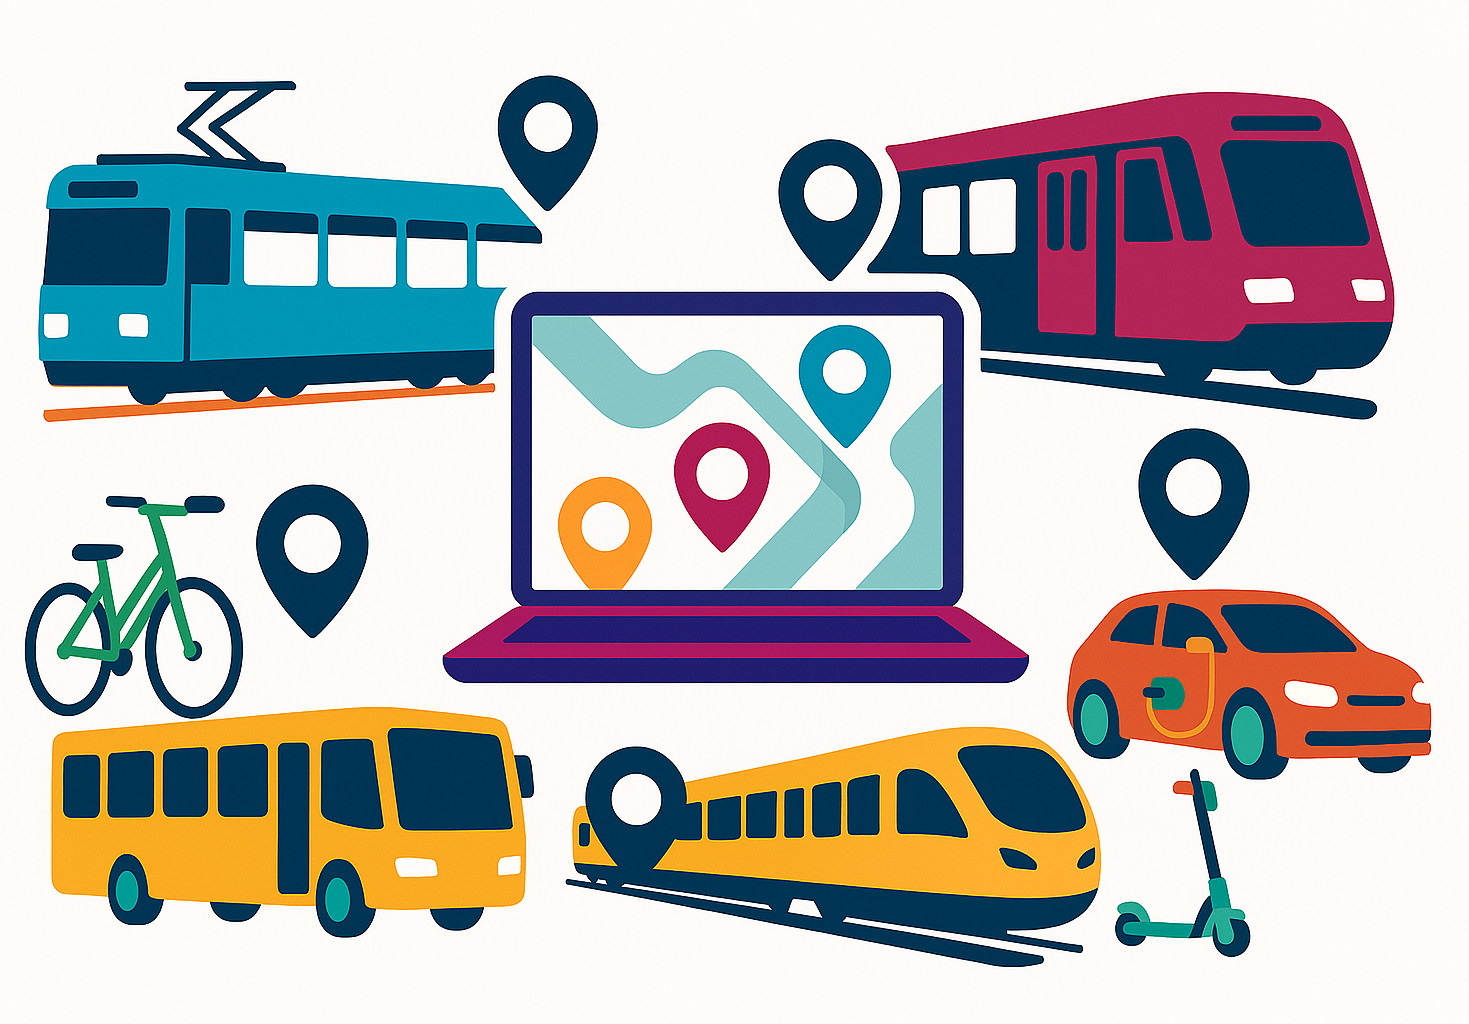
\includegraphics[width=0.8\textwidth]{Copertina}
\end{center}
\vspace{10mm}

{\large{\bf \noindent
Componenti del gruppo nr.2743:\\}
Bartocetti Enrico, matr. 0001115097\\
Benedetti Nicholas, matr. 0001114021\\
Tazzieri Nicolas, matr. 0001114078}

\end{titlepage}

\tableofcontents


\chapter{Analisi dei requisiti}

\section{Intervista iniziale}
Si vuole realizzare il software per la gestione del trasporto pubblico a lungo e corto raggio.
A seguito dell’intervista è stata prodotta la seguente descrizione delle specifiche del sistema in linguaggio naturale:
\\ \\
\textit{Le città di Vergineto, Urbania e San Giovanni in Marignano si sono accordate per avviare il progetto “Smart mobility 2030”, e richiedono un software per la gestione Smart e integrata del trasporto pubblico urbano ed extraurbano.}

\textit{Il sistema dovrà gestire diversi mezzi di TPL (Trasporto Pubblico Locale), quali bus, tram, metropolitana e treni ma in futuro potrebbe sorgere la necessità di aggiungerne di nuovi (ad esempio in seguito alla creazione di linee per i filobus). Ogni mezzo potrà percorrere diverse linee: ciò significa che un autobus utilizzato oggi per la linea 15, domani potrà percorrere la linea 21.}

\textit{Per ogni linea verranno effettuate delle fermate a orari prestabiliti. Potranno essere create anche linee straordinarie, ad esempio delle navette per eventi cittadini, di cui dovranno essere specificati periodo di validità, orari e fermate.}

\textit{Inoltre, per ridurre l’inquinamento nelle nostre città, verranno creati degli spazi riservati per lo sharing di biciclette, scooter e biciclette, e verranno aggiunte delle colonnine per la ricarica elettrica in modo da incentivare sia l’acquisto di auto elettriche sia l’utilizzo di monopattini o bici elettriche.}

\textit{Sarà disponibile una piattaforma online, nella quale si potranno visualizzare le diverse linee e le fermate che i mezzi effettuano con i relativi orari, nonché la disponibilità di posti liberi nelle aree di bikesharing e nelle colonnine elettriche. È anche prevista la registrazione di utenti “cittadini”, che potranno acquistare biglietti e abbonamenti. }

\textit{Un unico biglietto vale per tutti i mezzi di trasporto, e si vuole memorizzarne la durata, la data di convalida, la data di acquisto ed il titolare nel caso venga acquistato online: infatti un biglietto potrà anche essere acquistato da un fornitore fisico (ad esempio le tabaccherie della città). Sono presenti diverse tipologie di biglietti che differiscono in base alla durata dalla convalida e al prezzo. Gli abbonamenti sono biglietti che hanno una durata superiore ad un giorno.}

\textit{Si richiede anche la gestione dei dipendenti. In particolare, dovranno essere gestiti diversi autisti a cui verranno assegnati diversi mezzi in diversi slot orari. Sono inoltre presenti i controllori: in certi orari dovranno controllare diverse linee e saranno in grado di emettere multe. Gli orari e le linee da controllare vengono stabilite dal gestore delle linee di trasporto: ad esempio verranno prese in particolare considerazione quelle dove non ci sono molti incassi, ovvero dove è ipotizzabile una maggior evasione tariffaria, generando ingenti perdite economiche. Infine, l’amministratore del sistema potrà registrarsi in un portale specifico nel quale potrà gestire autisti, controllori e le linee. Inoltre, avrà la possibilità di visualizzare diverse statistiche riguardanti il sistema di trasporto, con enfasi particolare nei ricavi dei biglietti e nel tasso di evasione.}

\textit{Dovranno essere gestiti i lavori di manutenzione relativi a linee e mezzi per cui saranno specificati gli eventuali enti privati che li svolgeranno. Per le manutenzioni sarà richiesto di specificare una data di inizio e fine lavori, ed eventuali variazioni di servizio dovranno essere visualizzate al pubblico.}


\section{Prima fase di analisi}
Nell’analisi dell’intervista effettuata tempo addietro, abbiamo notato che il committente non è stato abbastanza esaustivo su alcuni argomenti.
Si è quindi resa necessaria un’ulteriore intervista per comprendere meglio il funzionamento di:
\begin{itemize}
	\item Sistema di acquisto e convalida di biglietti
	\item Gestione degli spazi speciali
	\item Gestione delle multe
\end{itemize}
\noindent Riportiamo le risposte R alle varie domande D.

\paragraph{D:}
“Come devono essere gestiti i biglietti, dal loro acquisto fino alla convalida?”
\\ {\bf R:} “I biglietti possono essere acquistati tramite il sito web, le biglietterie fisiche (sia dell’azienda sia da altri venditori autorizzati) e ticketmachine.
Ogni mezzo sarà dotato di una obliteratrice che, comunicando con il sistema informativo, alla lettura di un biglietto (tramite codice a barre stampato sul biglietto fisico o letto dal proprio dispositivo) ne controlla la validità e in caso affermativo lo registra come convalidato.”

\paragraph{D:}
“Cosa deve essere mostrato riguardo agli spazi per la mobilità sostenibile?”
\\ {\bf R:} “L’idea è quella di far vedere giusto una panoramica riguardo agli spazi.
In particolare, basta visualizzarne la posizione, l’indirizzo, un nome simbolico e quanti sono i posti rimanenti (quante biciclette rimanenti se si tratta di biciclette, quante colonnine se si tratta di colonnine elettriche, ecc.).
Inoltre, uno spazio può essere legato ad una fermata per rendere agevole il collegamento con aree non raggiunte dalle linee del TPL (es. appena scendo dal bus mi trovo nei pressi di una zona per il bike sharing)”

\paragraph{D:}
“Come funziona il sistema delle multe?”
\\ {\bf R:} “Le multe possono essere emesse dal personale qualificato a seguito di controlli effettuati sulle linee.
A ogni causale della multa corrisponde un certo importo base, a cui dovranno essere aggiunte eventuali penali per recidiva dell’utente o per ritardi nel pagamento.”


\section{Concetti principali}
Per rendere meglio fruibile la descrizione, abbiamo deciso di rimuovere eventuali ambiguità, seguendo la tabella qua sotto.

\begin{table}[h!]
\begin{tabular}{|l|l|}
\hline
\textbf{Termine} & \textbf{Nuovo Termine} \\
\hline
Mezzi di TPL & Mezzi di trasporto \\
Spazi riservati per il carsharing, … & Hub mobilità \\
Biglietti, Abbonamenti & Titolo di Viaggio \\
Gestore delle linee & Amministratore di Sistema \\
\hline
\end{tabular}
\end{table}

A seguito dell’intervista aggiuntiva è stata redatta la seguente descrizione del dominio in linguaggio naturale. Ambiguità e informazioni ridondanti sono state eliminate per garantire una miglior fruizione della descrizione:
\\ \\
Le città di Vergineto, Urbania e San Giovanni in Marignano si sono accordate per avviare il progetto “Smart mobility 2030”, e richiedono un software per la gestione Smart e integrata del trasporto pubblico urbano ed extraurbano.

Il sistema dovrà gestire diversi \underline{\texttt{mezzi di trasporto}}, quali \underline{\texttt{bus}}, \underline{\texttt{tram}}, \underline{\texttt{metropolitana}} e \underline{\texttt{treni}} lasciando la possibilità di aggiungerne altri in futuro. Ogni mezzo di trasporto potrà percorrere diverse \underline{\texttt{linee}}.

Una linea può essere \underline{\texttt{ordinaria}} o \underline{\texttt{straordinaria}}. Ogni linea effettua \underline{\texttt{fermate}} ad \underline{\texttt{orari}} prestabiliti. Per una linea straordinaria dovrà essere specificato il periodo di validità della linea.

Dovranno essere gestiti degli \underline{\texttt{hub mobilità}}, riservati per la ricarica elettrica e lo sharing di bici, monopattini e scooter. In particolare, si devono memorizzare la posizione, l’indirizzo, un nome simbolico e quanti sono i posti rimanenti. Inoltre, ad un hub mobilità può essere \underline{\texttt{associato}} ad una fermata.

Sarà disponibile una piattaforma online, nella quale si potranno visualizzare le diverse linee e le fermate che i mezzi effettuano con i relativi orari, nonché la disponibilità di posti liberi negli hub mobilità. È anche prevista la registrazione di \underline{\texttt{utenti cittadini}}, che potranno \underline{\texttt{acquistare}} \underline{\texttt{titoli di viaggio}}, che si dividono in \underline{\texttt{biglietti}} e \underline{\texttt{abbonamenti}}.

Un unico titolo di viaggio vale per tutti i mezzi di trasporto e vuole memorizzarne la durata, la data di convalida, la data di acquisto e l’utente cittadino associato nel caso sia un \underline{\texttt{biglietto digitale}}. Sono presenti diverse \underline{\texttt{tipologie}} di titoli di viaggio che differiscono in base alla durata dalla convalida e al prezzo. Gli abbonamenti sono biglietti che hanno una durata superiore ad un giorno. I biglietti possono essere acquistati anche in biglietterie fisiche e ticketmachine. Ogni mezzo di trasporto sarà dotato di una obliteratrice che, comunicando con il sistema informativo, alla lettura di un biglietto ne controlla la validità, e in caso affermativo, lo registra come \underline{\texttt{convalidato}}.

Si richiede anche la gestione dei \underline{\texttt{dipendenti}}. Essi si dividono in \underline{\texttt{Autisti}}, \underline{\texttt{Controllori}} e \underline{\texttt{Amministratori di sistema}}. Agli Autisti a verranno assegnati diversi mezzi di trasposto in slot orari diversi. I controllori dovranno controllare diverse linee negli slot orari assegnati, e saranno in grado di emettere \underline{\texttt{multe}}.  A ogni \underline{\texttt{causale della multa}} corrisponde un certo importo base, a cui potranno essere aggiunte eventuali penali per recidiva dell’utente o per ritardi nel pagamento. Gli orari e le linee da controllare vengono stabilite dall’amministratore di sistema. Infine, l’amministratore del sistema potrà registrarsi in un portale specifico nel quale potrà gestire autisti, controllori e le linee. Inoltre, avrà la possibilità di visualizzare diverse statistiche riguardanti il sistema di trasporto, con enfasi particolare nei ricavi dei titoli di viaggio e nel tasso di evasione.

Dovranno essere gestiti i lavori di \underline{\texttt{manutenzione}}, che possono coinvolgere \underline{\texttt{linee}} e \underline{\texttt{mezzi di trasporto}}, per cui saranno specificati gli eventuali \underline{\texttt{enti privati}} che li svolgeranno. Per le manutenzioni sarà richiesto di specificare una data di inizio e fine lavori, ed eventuali \underline{\texttt{variazioni di servizio}} che coinvolgono linee dovranno essere visualizzate al pubblico.

\chapter{Progettazione Concettuale}
\section{Schema Scheletro}
\section{Raffinamenti Proposti}
\section{Schema Concettuale Finale}

\chapter{Progettazione Logica}
\section{Stima del volume dei dati}
Per poter gestire al meglio il carico di lavoro della base di dati, insieme al committente si è creata una stima del volume dei dati per entità e associazioni che il database dovrà gestire, di cui se ne riportano i numeri nella Tabella \ref{table:volumeDati}.
La stima è valida per un carico di lavoro di circa 6 mesi.

\begin{longtable}{|p{7.5cm}|r|c|}
\caption{Stima del volume dei dati}
\label{table:volumeDati}\\
\hline
\textbf{NOME} & \textbf{VOLUME STIMATO} & \textbf{E/A} \\
\hline
\endhead

ABBONAMENTO & 30.000 & E \\
\hline
AMMINISTRATIVO & 10 & E \\
\hline
ATTUAZIONE CORSA & 250.000 & E \\
\hline
AUMENTO & 10 & E \\
\hline
AUTISTA & 130 & E \\
\hline
AZIENDA & 15 & E\\
\hline
BIGLIETTO DIGITALE & 150.000 & E \\
\hline
BIGLIETTO FISICO & 150.000 & E \\
\hline
CAUSALE MULTA & 10 & E \\
\hline
CONTENUTO HUB & 4 & E \\
\hline
CONTROLLORE & 40 & E \\
\hline
DIPENDENTE & 180 & E \\
\hline
FERMATA & 450 & E \\
\hline
HUB MOBILITÀ & 225 & E \\
\hline
LINEA & 75 & E \\
\hline
MANUTENZIONE & 50 & E \\
\hline
MANUTENZIONE LINEA & 10 & E \\
\hline
MANUTENZIONE MEZZO & 40 & E \\
\hline
MEZZO & 160 & E \\
\hline
MULTA & 10.000 & E \\
\hline
ORARIO LINEA & 1500 & E \\
\hline
ORDINARIA & 65 & E \\
\hline
PERSONA & 20.000 & E \\
\hline
STRAORDINARIA & 10 & E \\
\hline
TARIFFA ABBONAMENTO & 5 & E \\
\hline
TARIFFA BIGLIETTO & 10 & E \\
\hline
TIPOLOGIA MEZZO & 4 & E \\
\hline
TITOLO DI VIAGGIO & 750.000 & E \\
\hline
TRATTA & 1.000 & E \\
\hline
UTENTE & 10.000 & E \\
\hline
ACQUISTO ABBONAMENTO & 30.000 & A \\
\hline
ACQUISTO BIGLIETTO & 150.000 & A \\
\hline
ARRIVO & 1.000 & A \\
\hline
ASSUNZIONE & 160 & A \\
\hline
CONDUCENTE & 250.000 & A \\
\hline
CONTENUTO & 450 & A \\
\hline
CONTROLLO & 50.000 & A \\
\hline
CONVALIDA & 200.000 & A \\
\hline
EFFETTUAZIONE & 250.000 & A \\
\hline
EMISSIONE & 10.000 & A \\
\hline
FASCIA ABBONAMENTO & 30.000 & A \\
\hline
FASCIA BIGLIETTO & 300.000 & A \\
\hline
IMPIEGO & 250.000 & A \\
\hline
INCARICO & 25 & A \\
\hline
INCREMENTO & 10 & A \\
\hline
INTESTAZIONE & 10.000 & A \\
\hline
MODIFICA & 10 & A \\
\hline
NECESSITA & 40 & A \\
\hline
PARTENZA & 1.000 & A \\
\hline
PRESENZA & 165 & A \\
\hline
RIFERIMENTO & 10.000 & A \\
\hline
SOSTITUZIONE & 10 & A \\
\hline
SPECIFICAZIONE & 1.500 & A \\
\hline
TIPO LINEA & 75 & A \\
\hline
TIPOLOGIA & 10.000 & A \\
\hline
TRAGITTO & 1.500 & A \\
\hline
\end{longtable}


\section{Descrizione operazioni}
Riportiamo in Tabella \ref{table:operazioni} le principali operazioni che saranno svolte sulla base di dati, marcando con un asterisco (*) le operazioni di cui è necessario calcolare i costi dati da attributi ridondanti.

\begin{longtable}{|c|p{9cm}|c|l|l|}
\caption{Numero stimato di operazioni per settimana, con tipo di utente che le effettua}
\label{table:operazioni}\\
\hline
\textbf{\#} & \textbf{Operazione} & \textbf{Op / 7gg} & \textbf{Tipo Utente} \\
\hline
\endhead
1*  & \hyperref[op1]{Visualizzazione di tutte le linee attive} & 4.000 & Tutti **** \\
\hline
2 & \hyperref[op2]{Visualizzazione fermate e orari di una linea} & 3.500 & Tutti **** \\
\hline
3 & \hyperref[op3]{Visualizzazione degli hub mobilità} & 500 & Tutti \\
\hline
4* & \hyperref[op4]{Visualizzazione orario e mezzo assegnato} & 150 & Autista ***** \\
\hline
5* & \hyperref[op5]{Visualizzazione orario e linee assegnate} & 100 & Controllore ***** \\
\hline
6 & \hyperref[op6]{Estrazione delle linee con più convalide nell'ultimo mese} & 3 & Amministratore *****  \\
\hline
7 & \hyperref[op7]{Estrazione delle manuntenzioni che coinvolgono un determinato mezzo} & 5 & Amministratore \\
\hline
8 & \hyperref[op8]{Estrazione delle manuntenzioni ed eventuali linee sostitutive che coinvolgono una linea} & 5 & Amministratore ***** \\
\hline
9 & \hyperref[op9]{Visualizzazione incassi dati dalle convalide per una linea} & 10 & Amministratore **** \\
\hline
10 & \hyperref[op10]{Estrazione degli incassi per tipo di titolo in periodo definito} & 5 & Amministratore \\
\hline
11 & \hyperref[op11]{Estrazione delle linee con più multe negli ultimi 3 mesi} & 2 & Amministratore ***** \\
\hline
12 & \hyperref[op12]{Estrazione delle 5 linee con manutenzioni più gravose (in termini linee sostitutive e durata)} & 2 & Amministratore *****  \\
\hline
13 & \hyperref[op13]{Estrazione delle linee con \textgreater 5 controlli/giorno e \textless = 10 multe/giorno} & 3 & Amministratore  \\
\hline
14* & \hyperref[op14]{Visualizzazione delle linee con il maggior tempo di percorrenza} & 2 & Amministratore ***** \\
\hline
15 & \hyperref[op15]{Estrazione delle linee con più hub mobilità lungo il percorso} & 3 & Amministratore ***** \\
\hline
16 & \hyperref[op16]{Media di soldi spesi in multe per persona} & 2 & Amministratore \\
\hline
17 & \hyperref[op17]{Visualizzazione delle aziende che non hanno effettuato nessuna manutenzione nell'ultimo mese} & 4 & Amministratore \\
\hline
18 & \hyperref[op18]{Visualizzazione delle fermate in cui è presente un hub mobilità contenente tutti i tipi di servizi green} & 1 & Amministratore \\
\hline
19* & \hyperref[op19]{Inserimento di una variazione di servizio} & 1 & Amministratore ***** \\
\hline
20* & \hyperref[op20]{Aggiunta di una tratta a una linea esistente} & 1 & Amministratore ***** \\
\hline
21* & \hyperref[op21]{Creazione di una nuova linea} & 1 & Amministratore ***** \\
\hline
\end{longtable}

\section{Analisi delle operazioni}
Indichiamo con:
\begin{itemize}
	\item ${C_{tot}}$ il costo totale dell'operazione.
	\item ${O_{settimana}}$ il numero di volte che l'operazione verrà eseguita in una settimana
	\item ${A_{scrittura}}$ il numero di accessi in scrittura effettuato da un'operazione
	\item ${A_{lettura}}$ il numero di accessi in lettura effettuato da un'operazione
\end{itemize}

\noindent Di seguito eseguiamo l'analisi delle operazioni presenti in Tabella \ref{table:operazioni}, riportando lo schema di navigazione, la tabella degli accessi e il calcolo del costo della specifica operazione per ogni settimana.
\begin{enumerate}[label=\textbf{\arabic*)}]

  % -------------------------------------------------------------------------------------------------------------------------------------------
  % ------------------------------------------------------------------------------------------------------------------------------------------- 

   \item \textbf{Visualizzazione di tutte le linee attive} \label{op1} \\
    \[ {O_{settimana} = 4.000} \]
    Questa operazione serve per visualizzare tutte le linee che sono in funzione (ovvero non risultano in manutenzione) al momento attuale. Poiché è presente l'attributo ridondante  \texttt{attiva} che potrebbe velocizzare lo svolgimento delle operazioni, viene eseguito il calcolo degli accessi sia tenendo conto della presenza dell'attributo, sia senza.\\
    Si vuole quindi selezionare:
    \begin{itemize}
	\renewcommand\labelitemi{--}
    \item Il codice della \texttt{LINEA}
    \item La prima e l'ultima \texttt{FERMATA}
    \item Il nome della \texttt{TIPOLOGIA MEZZO} utilizzato
    \end{itemize}  
    
    \begin{itemize}
    \item \textbf{Analisi con attributo ridondante \texttt{attiva} su \texttt{ORDINARIA}}
    \begin{center}
    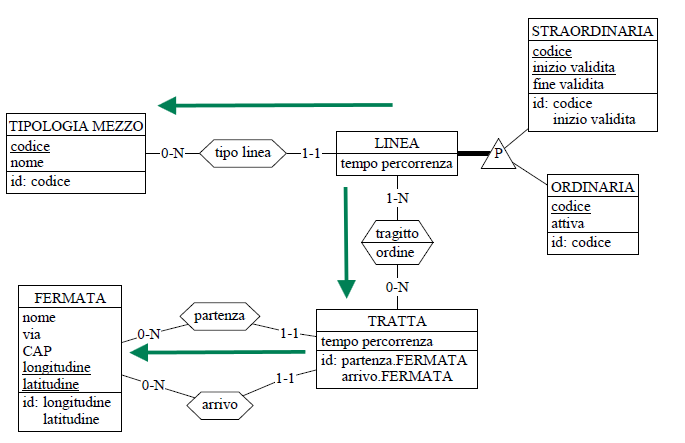
\includegraphics[width=0.7\textwidth]{VisualLineeRid}
    \end{center}
    \begin{table}[H]
    \centering
    \begin{tabular}{|c|c|l|l|}
    \hline
    \textbf{Nome} & \textbf{Tipo} & \textbf{Numero accessi} & \textbf{S/L} \\
    \hline
    LINEA & E & 75 & L \\
    \hline
    TIPOLOGIA MEZZO & E & 75 & L \\
    \hline
    TRAGITTO & A & 1.500 & L \\
    \hline
    TRATTA & E & 150 & L \\
    \hline
    FERMATA (PARTENZA) & E & 75 & L \\
    \hline
    FERMATA (ARRIVO) & E & 75 & L \\
    \hline
    \multicolumn{4}{c}{\textbf{Totale}} \\    
    \multicolumn{4}{c}{${A_{lettura}}$ = 1.950, ${A_{scrittura}}$ = 0} \\
    \hline
    \end{tabular}
    \end{table}
    \begin{center}
    ${C_{tot} = {O_{settimana}}\cdot{A_{lettura}}= 7.800.000}$
    \end{center}

    \item \textbf{Analisi senza attributo ridondante \texttt{attiva} su \texttt{ORDINARIA}}
    \begin{center}
    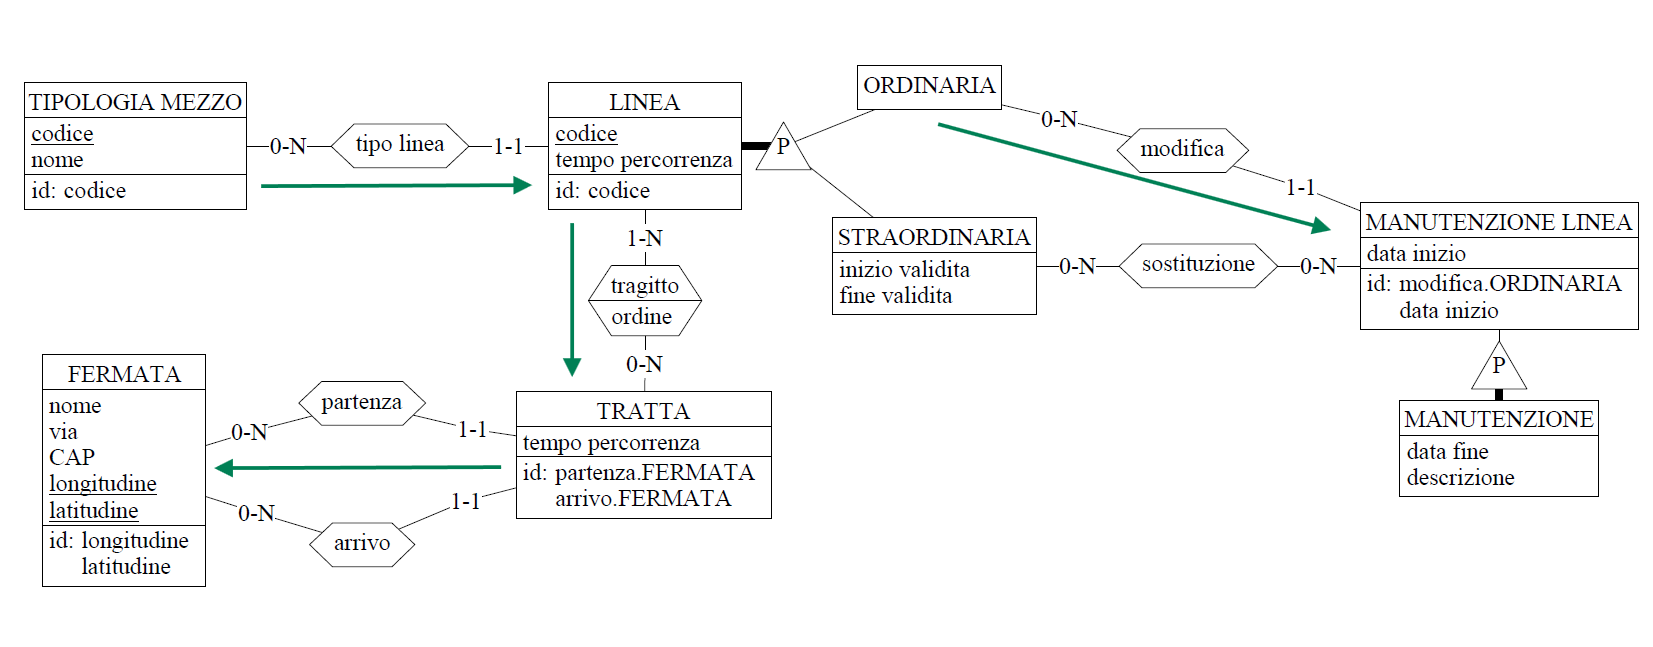
\includegraphics[width=0.9\textwidth]{VisualLineeNoRid}
    \end{center}
    \begin{table}[H]
    \centering
    \begin{tabular}{|c|c|l|l|}
    \hline
    \textbf{Nome} & \textbf{Tipo} & \textbf{Numero accessi} & \textbf{S/L} \\
    \hline
    LINEA & E & 75 & L \\
    \hline
    MANUTENZIONE LINEA & E & 10 & L \\
    \hline
    TIPOLOGIA MEZZO & E & 75 & L \\
    \hline
    TRAGITTO & A & 1.500 & L \\
    \hline
    TRATTA & E & 150 & L \\
    \hline
    FERMATA (PARTENZA) & E & 75 & L \\
    \hline
    FERMATA (ARRIVO) & E & 75 & L \\
    \hline
    \multicolumn{4}{c}{\textbf{Totale}} \\    
    \multicolumn{4}{c}{${A_{lettura}}$ = 1.960, ${A_{scrittura}}$ = 0} \\
    \hline
    \end{tabular}
    \end{table}
    \begin{center}
    ${C_{tot} = {O_{settimana}}\cdot{A_{lettura}}= 7.840.000}$
    \end{center}
    \end{itemize}

  % ------------------------------------------------------------------------------------------------------------------------------------------- 
  % ------------------------------------------------------------------------------------------------------------------------------------------- 

        \item \textbf{Visualizzazione fermate e orari di una linea} \label{op2} \\
        \[ {O_{settimana} = 3.500} \]
        Dobbiamo visualizzare le linee, i suoi orari e le fermate fatte da essa per qualsiasi utente.
        \begin{center}
	    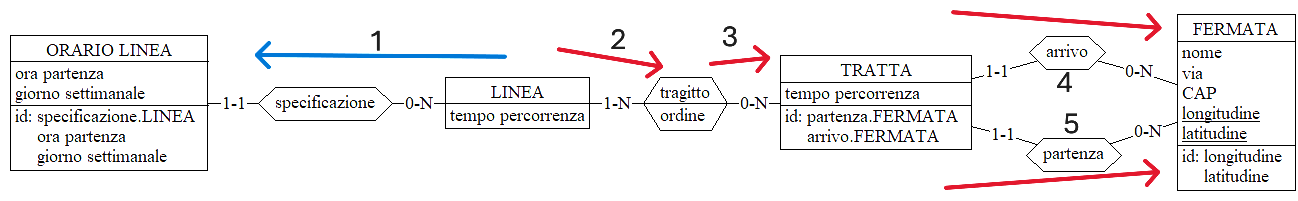
\includegraphics[width=0.9\textwidth]{op_2}
	    \end{center}
        \begin{table}[H]
	\centering
        \begin{tabular}{|c|c|l|l|}
        \hline
        \textbf{Nome} & \textbf{Tipo} & \textbf{Numero accessi} & \textbf{S/L} \\
        \hline
        LINEA & E & 1 & L \\
        \hline
        ORARIO LINEA & E & 20 & L \\
        \hline
        TRAGITTO & A & 20 & L \\
        \hline
        TRATTA & E & 20 & L \\
        \hline
        FERMATA & E & 40 & L \\
        \hline
        \multicolumn{4}{c}{\textbf{Totale}} \\    
        \multicolumn{4}{c}{${A_{lettura}}$ = 71, ${A_{scrittura}}$ = 0} \\
        \hline
        \end{tabular}
        \end{table}
        \begin{center}
        ${C_{tot} = {O_{settimana}}\cdot{A_{lettura}} = 248.500}$
        \end{center}

  % -------------------------------------------------------------------------------------------------------------------------------------------
  % ------------------------------------------------------------------------------------------------------------------------------------------- 

        \item \textbf{Visualizzazione degli hub mobilità} \label{op3} \\
	\[{O_{settimana} = 500}\]
	Questa operazione deve poter essere fatta da qualsiasi persona che accede all'applicativo. Si richiede per ogni \texttt{HUB MOBILITA} di visualizzare:
	\begin{itemize}
	\renewcommand\labelitemi{--}
	    \item Tutti gli attributi di \texttt{HUB MOBILITA}
	    \item I tipi di \texttt{CONTENUTO HUB} per ogni \texttt{HUB MOBILITA}
	    \item I posti rimanenti per ogni \texttt{CONTENUTO HUB} nell'\texttt{HUB MOBILITA}
	    \item L'eventuale fermata a cui è collegato
	\end{itemize}
	\begin{center}
	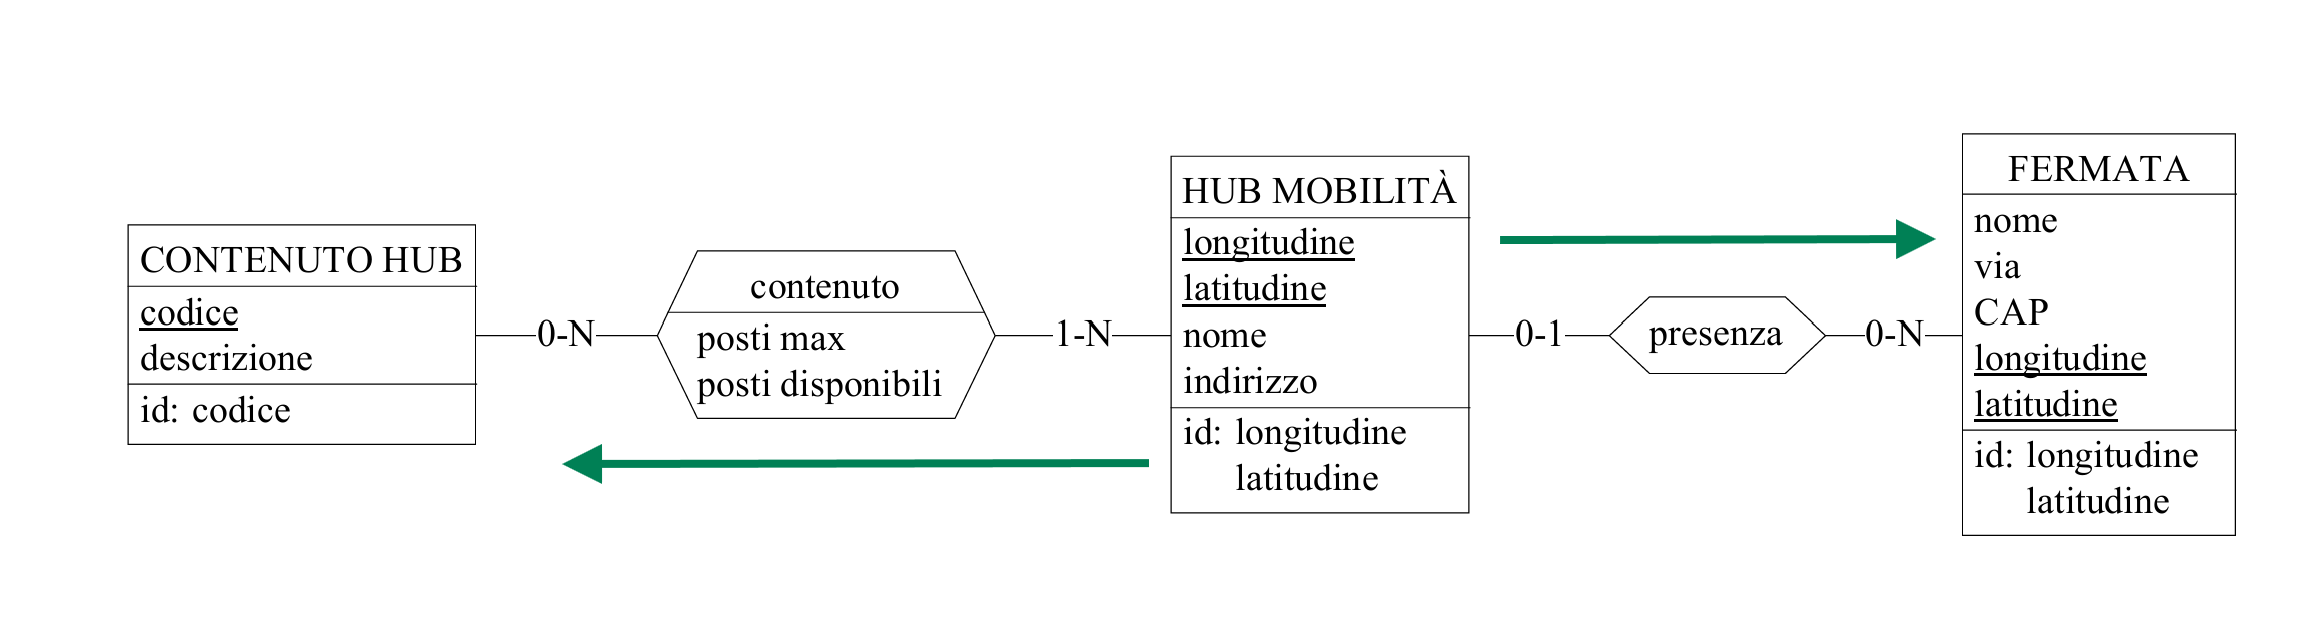
\includegraphics[width=0.9\textwidth]{VisualHubMobilita}
	\end{center}
    \begin{table}[H]
    \centering
	\begin{tabular}{|l|c|c|c|}
	\hline
	Nome & Tipo & Numero Accessi & S/L \\
	\hline
	HUB MOBILITA & E & 225 & L \\
	\hline
	CONTENUTO & A & 225 $\times$ 2 & L \\
	\hline
	CONTENUTO HUB & E & 225 $\times$ 2 & L \\
	\hline
	FERMATA & E & 165 & L \\
	\hline
        \multicolumn{4}{c}{\textbf{Totale}} \\    
        \multicolumn{4}{c}{${A_{lettura}}$ = 1290, ${A_{scrittura}}$ = 0} \\
        \hline
	\end{tabular}
    \end{table}	
    \begin{center}
    ${C_{tot} = {O_{settimana}}\cdot{A_{lettura}}= 645.000}$
    \end{center}

  % -------------------------------------------------------------------------------------------------------------------------------------------
  % ------------------------------------------------------------------------------------------------------------------------------------------- 

         \item \textbf{Visualizzazione orario e linee assegnate agli autisti} \label{op4} \\
            \[ {O_{settimana} = 150} \]
           \begin{itemize}
            \item \textbf{Analisi con attributo ridondante \texttt{tempo percorrenza} su \texttt{LINEA}} \\
            Dobbiamo visualizzare l'orario di lavoro di un autista, mostrando la linea l'orario e il mezzo assegnato.
            La lettura partirà da un autista; il numero di letture è stato calcolato dividendo il numero totale delle entità attuazione corsa (250.000) con il numero totale degli autisti (130), in modo da trovare la media di associazioni per ogni autista.
            \begin{center}
	        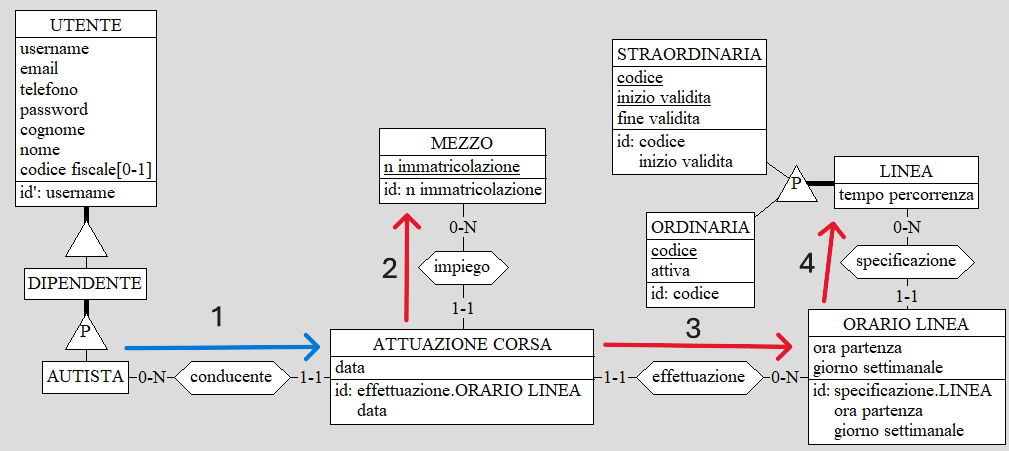
\includegraphics[width=0.9\textwidth]{op_4_RID}
	        \end{center}
            \begin{table}[H]
            \centering
            \begin{tabular}{|c|c|l|l|}
            \hline
            \textbf{Nome} & \textbf{Tipo} & \textbf{Numero accessi} & \textbf{S/L} \\
            \hline
            AUTISTA & E & 1 & L \\
            \hline
            ATTUAZIONE CORSA & E & 1923 & L \\ 
            \hline
            ORARIO LINEA & E & 1923 & L \\ 
            \hline
            LINEA & E & 1923 & L \\
            \hline
            MEZZO & E & 1923 & L \\
            \hline
            \multicolumn{4}{c}{\textbf{Totale}} \\    
            \multicolumn{4}{c}{${A_{lettura}}$ = 7693, ${A_{scrittura}}$ = 0} \\
            \hline
            \end{tabular}
            \end{table}
            \begin{center}
            ${C_{tot} = {O_{settimana}}\cdot {A_{lettura}} =1.153.950}$
            \end{center}

            \item \textbf{Analisi senza attributo ridondante \texttt{tempo percorrenza} su \texttt{LINEA}} \\
            Dobbiamo visualizzare l'orario di lavoro di un autista, mostrando la linea l'orario e il mezzo assegnato.
            La lettura partirà da un autista, le letture sono state calcolate nello stesso modo.\\
            Visto che non abbiamo il tempo di percorrenza su \texttt{LINEA}, dobbiamo ricavarlo tramite le varie \texttt{TRATTE} che compongono la linea. Ogni \texttt{LINEA} ha in media 20 associazioni \texttt{TRAGITTO}.
            \begin{center}
	        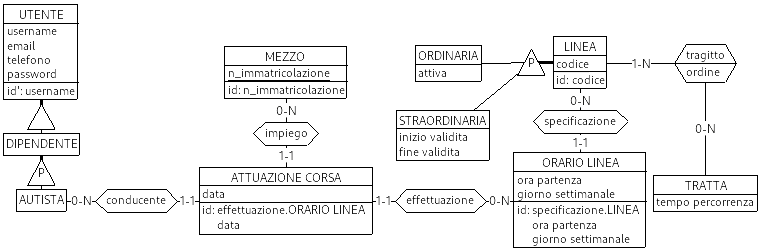
\includegraphics[width=0.9\textwidth]{op_4_NORID}
	        \end{center}
            \begin{table}[H]
            \centering
            \begin{tabular}{|c|c|l|l|}
            \hline
            \textbf{Nome} & \textbf{Tipo} & \textbf{Numero accessi} & \textbf{S/L} \\
            \hline
            AUTISTA & E & 1 & L \\
            \hline
            ATTUAZIONE CORSA & E & 1.923 & L \\ 
            \hline
            ORARIO LINEA & E & 1.923 & L \\ 
            \hline
            MEZZO & E & 1.923 & L \\
            \hline
            LINEA & E & 1.923 & L \\
            \hline
            TRAGITTO & A & 38.460 & L \\
            \hline
            TRATTA & E & 38.460 & L \\
            \hline 
            \multicolumn{4}{c}{\textbf{Totale}} \\    
            \multicolumn{4}{c}{${A_{lettura}}$ = 84.613, ${A_{scrittura}}$ = 0} \\
            \hline
            \end{tabular}
            \end{table}
            \begin{center}
            ${C_{tot} = {O_{settimana}}\cdot {A_{lettura}} =12.691.950}$
            \end{center}
    \end{itemize}


  % ------------------------------------------------------------------------------------------------------------------------------------------- 
  % ------------------------------------------------------------------------------------------------------------------------------------------- 

    \item \textbf{Visualizzazione orario e linee assegnate ai controllori} \label{op5} \\
    \[ {O_{settimana} = 100} \]
    Questa operazione serve a un controllore per visualizzare il suo orario di lavoro e come dovrà essere svolto (ovvero le linee che dovrà controllare). Poiché è necessario calcolare l'orario di arrivo della linea, l'attributo \texttt{tempo percorrenza} su \texttt{LINEA} rende superfluo il calcolo del tempo tramite la somma dei tempi di tutte le \texttt{TRATTA}: è quindi necessario eseguire i calcoli dei costi con attributo ridondante e non. \\
    Nei conti terremo conto del fatto che l'operazione è relativa a un solo giorno, ovvero sarà eseguito un filtro delle \texttt{ATTUAZIONE CORSA}. \\ 
    Dati un controllore e una data, bisogna quindi visualizzare:
    \begin{itemize}
    \renewcommand\labelitemi{--}
    \item L'orario di partenza, di arrivo e il codice della \texttt{LINEA} da controllare
    \item Il numero di immatricolazione del \texttt{MEZZO} che effettua la corsa
    \end{itemize}
	
    \begin{itemize}
    \item \textbf{Analisi con attributo ridondante \texttt{tempo percorrenza} su \texttt{LINEA}}
    \begin{center}
    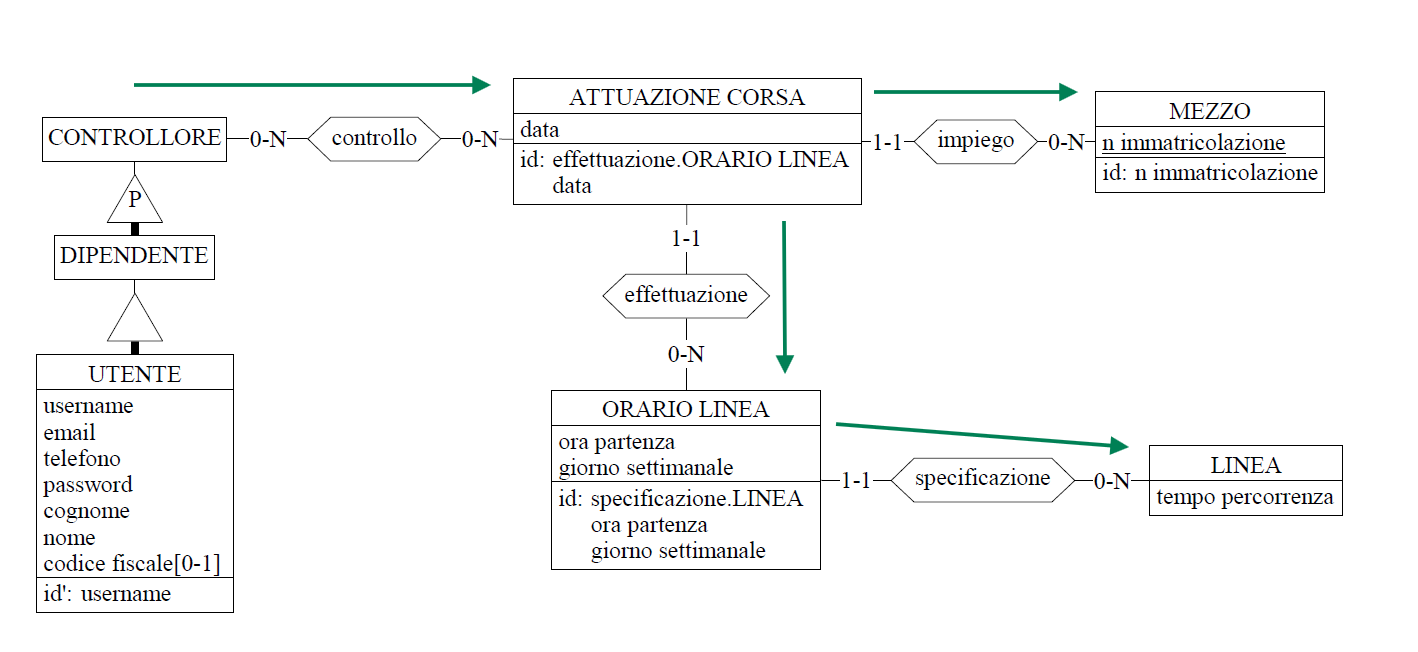
\includegraphics[width=0.9\textwidth]{VisualOrarioControlloriRid}
    \end{center}
    \begin{table}[H]
    \centering
    \begin{tabular}{|c|c|l|l|}
    \hline
    \textbf{Nome} & \textbf{Tipo} & \textbf{Numero accessi} & \textbf{S/L} \\
    \hline
    CONTROLLORE & E & 1 & L \\
    \hline
    CONTROLLO & A & 1.250 & L \\
    \hline
    ATTUAZIONE CORSA & E & 1.250 & L \\
    \hline
    ORARIO LINEA & E & 7 & L \\
    \hline
    LINEA & E & 7 & L \\
    \hline
    MEZZO & E & 7 & L \\
   \hline
    \multicolumn{4}{c}{\textbf{Totale}} \\    
    \multicolumn{4}{c}{${A_{lettura}}$ = 2.522, ${A_{scrittura}}$ = 0} \\
    \hline
    \end{tabular}
    \end{table}
    \begin{center}
    ${C_{tot} = {O_{settimana}}\cdot{A_{lettura}}= 252.200}$
    \end{center}

    \item \textbf{Analisi senza attributo ridondante \texttt{tempo percorrenza} su \texttt{LINEA}}
    \begin{center}
    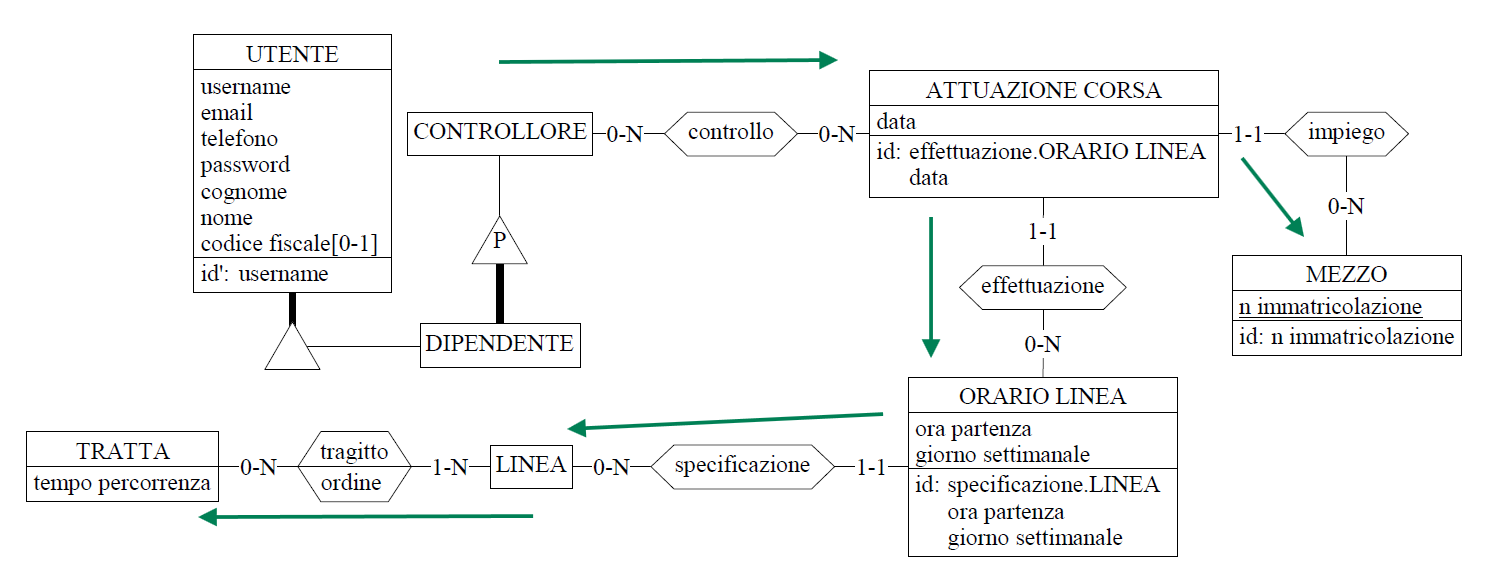
\includegraphics[width=0.9\textwidth]{VisualOrarioControlloriNoRid}
    \end{center}
    \begin{table}[H]
    \centering
    \begin{tabular}{|c|c|l|l|}
    \hline
    \textbf{Nome} & \textbf{Tipo} & \textbf{Numero accessi} & \textbf{S/L} \\
    \hline
    CONTROLLORE & E & 1 & L \\
    \hline
    CONTROLLO & A & 1.250 & L \\
    \hline
    ATTUAZIONE CORSA & E & 1.250 & L \\
    \hline
    ORARIO LINEA & E & 7 & L \\
    \hline
    LINEA & E & 7 & L \\
    \hline
    TRAGITTO & A & 140 & L \\
    \hline
    TRATTA & E & 140 & L \\
    \hline
    MEZZO & E & 7 & L \\
   \hline
    \multicolumn{4}{c}{\textbf{Totale}} \\    
    \multicolumn{4}{c}{${A_{lettura}}$ = 2.802, ${A_{scrittura}}$ = 0} \\
    \hline
    \end{tabular}
    \end{table}
    \begin{center}
    ${C_{tot} = {O_{settimana}}\cdot{A_{lettura}}= 280.200}$
    \end{center}
    \end{itemize}

  % ------------------------------------------------------------------------------------------------------------------------------------------- 
  % ------------------------------------------------------------------------------------------------------------------------------------------- 

    \item \textbf{Estrazione delle linee con più convalide nell'ultimo mese} \label{op6} \\
    \[ {O_{settimana} = 3} \]
    Dobbiamo estrarre le linee con più biglietti convalidati nell'ultimo mese. Il conteggio per la quantità di letture su \texttt{CONVALIDA} è stato fatto con una media tramite la tabella dei volumi. 
    \begin{center}
	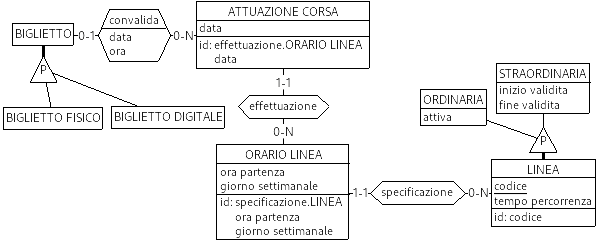
\includegraphics[width=0.9\textwidth]{op_6}
	\end{center}
    \begin{table}[H]
    \centering
    \begin{tabular}{|c|c|l|l|}
    \hline
    \textbf{Nome} & \textbf{Tipo} & \textbf{Numero accessi} & \textbf{S/L} \\
    \hline
    ATTUAZIONE CORSA & E & 250.000 & L \\
    \hline
    CONVALIDA & E & 33.333 & L \\ 
    \hline
    ORARIO LINEA & E & 1 & L \\ 
    \hline
    LINEA & E & 1 & L \\ 
    \hline
    \multicolumn{4}{c}{\textbf{Totale}} \\    
    \multicolumn{4}{c}{${A_{lettura}}$ = 283.335, ${A_{scrittura}}$ = 0} \\
    \hline
    \end{tabular}
    \end{table}
    \begin{center}
    ${C_{tot} = {O_{settimana}}\cdot {A_{lettura}} = 850.005}$
    \end{center}

  % ------------------------------------------------------------------------------------------------------------------------------------------- 
  % ------------------------------------------------------------------------------------------------------------------------------------------- 

    \item \textbf{Estrazione delle manuntenzioni che coinvolgono un determinato mezzo} \label{op7} \\
    \[ {O_{settimana} = 5} \]
    Questa operazione serve per visualizzare tutte le manutenzioni che sono state effettuate ad un mezzo.\\
    Dato un mezzo bisogna quindi visualizzare:
    \begin{itemize}
    \renewcommand\labelitemi{--}
    \item Tutti i dati della \texttt{MANUTENZIONE}
    \item La partita iva dell'eventuale \texttt{AZIENDA} esterna incaricata della manutenzione
    \end{itemize}  
    \begin{center}
    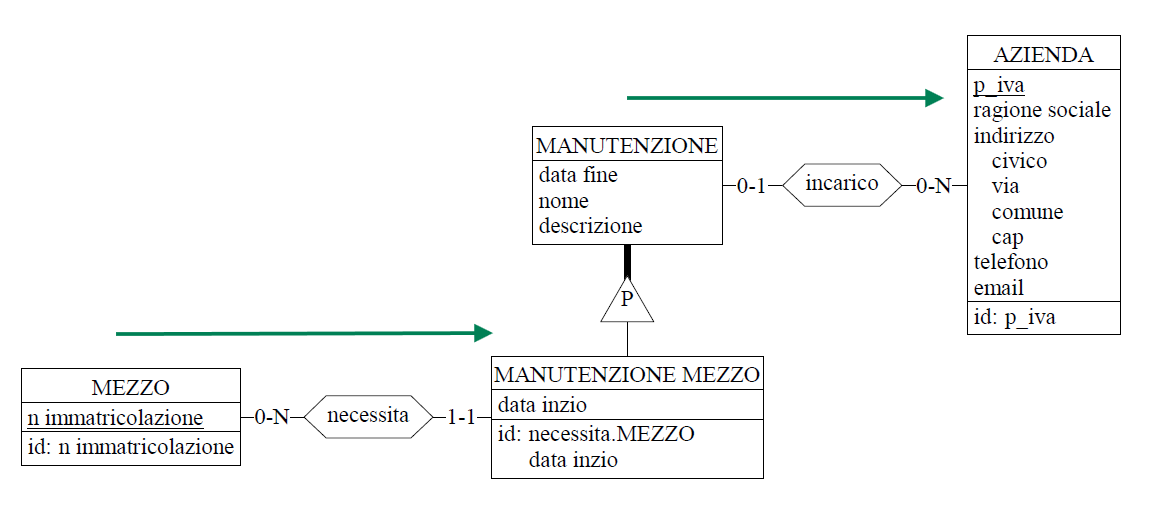
\includegraphics[width=0.8\textwidth]{VisualManutenzioniMezzo}
    \end{center}
    \begin{table}[H]
    \centering
    \begin{tabular}{|c|c|l|l|}
    \hline
    \textbf{Nome} & \textbf{Tipo} & \textbf{Numero accessi} & \textbf{S/L} \\
    \hline
    MEZZO & E & 1 & L \\
    \hline
    MANUTENZIONE MEZZO & E & 4 & L \\
    \hline
    AZIENDA & E & 2 & L \\
    \hline
    \multicolumn{4}{c}{\textbf{Totale}} \\    
    \multicolumn{4}{c}{${A_{lettura}}$ = 7, ${A_{scrittura}}$ = 0} \\
    \hline
    \end{tabular}
    \end{table}
    \begin{center}
    ${C_{tot} = {O_{settimana}}\cdot{A_{lettura}}= 35}$
    \end{center}

  % ------------------------------------------------------------------------------------------------------------------------------------------- 
  % ------------------------------------------------------------------------------------------------------------------------------------------- 

    \item \textbf{Estrazione delle manuntenzioni ed eventuali linee sostitutive che coinvolgono una linea (Variazioni di servizio)} \label{op8} \\
	\[{O_{settimana} = 5}\]
	Questa operazione deve poter essere effettuata da qualsiasi utente. Consente di visualizzare le variazioni di servizio di una specifica linea.\\
	Specificata una linea, va estratto:
	\begin{itemize}
	\renewcommand\labelitemi{--}
	    \item Tutti gli attributi di \texttt{MANUNTENZIONE LINEA} e \texttt{MANUNTENZIONE}
	    \item L'azienda che effettua la manuntezione
	    \item Tutte le linee straordinarie (codice, inizioValidita, fineValidita, partenza, arrivo) con cui viene sostituita la linea
	\end{itemize}
	
	\begin{center}
	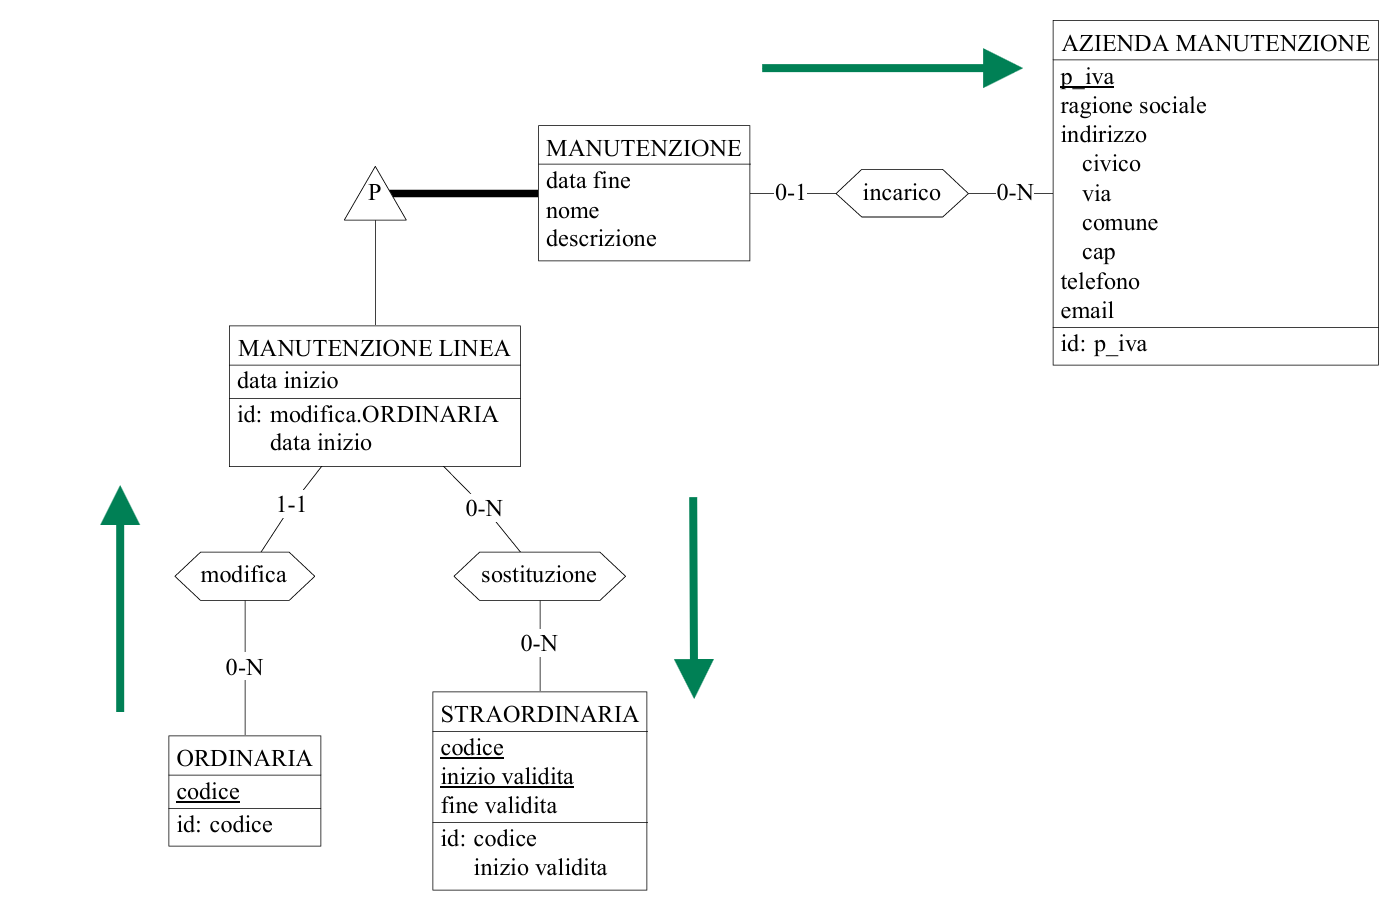
\includegraphics[width=0.8\textwidth]{VisualManunLinee}
	\end{center}
	\begin{table}[H]
	\centering
	\begin{tabular}{|l|c|c|c|}
	\hline
	Nome & Tipo & Numero Accessi & S/L \\
	\hline
	ORDINARIA & E & 1 & L \\
	\hline
	MANUNTENZIONE LINEA & E & 10 & L \\
	\hline
	AZIENDA & E & 10 & L \\
	\hline
	SOSTITUZIONE & A & 1 $\times$ 10 & L \\
	\hline
	STRAORDINARIA & E & 1 $\times$ 10 & L \\
          \hline
          \multicolumn{4}{c}{\textbf{Totale}} \\    
          \multicolumn{4}{c}{${A_{lettura}}$ = 41, ${A_{scrittura}}$ = 0} \\
          \hline
	\end{tabular}
	\end{table}
	    \begin{center}
	    ${C_{tot} = {O_{settimana}}\cdot{A_{lettura}}= 205}$
	    \end{center}

  % ------------------------------------------------------------------------------------------------------------------------------------------- 
  % ------------------------------------------------------------------------------------------------------------------------------------------- 

	\item \textbf{Visualizzazione incassi dati dalle convalide per una linea} \label{op9} \\
    \[ {O_{settimana} = 10} \]
    Partendo da una linea dobbiamo visualizzare gli incassi fatti da essa tramite i biglietti convalidati.
    \begin{center}
	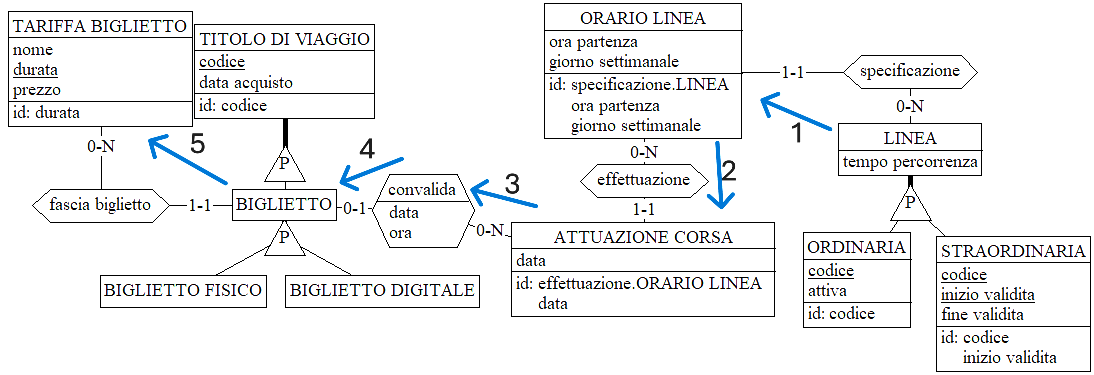
\includegraphics[width=0.9\textwidth]{op_9}
	\end{center}
    \begin{table}[H]
    \centering
    \begin{tabular}{|c|c|l|l|}
    \hline
    \textbf{Nome} & \textbf{Tipo} & \textbf{Numero accessi} & \textbf{S/L} \\
    \hline
    LINEA & E & 1 & L \\ 
    \hline
    ORARIO LINEA & E & 20 & L \\ 
    \hline
    ATTUAZIONE CORSA & E & 167 & L \\
    \hline
    CONVALIDA & A & 209 & L \\
    \hline
    BIGLIETTO & E & 209 & L \\
    \hline
    TARIFFA BIGLIETTO & E & 209 & L \\
    \hline
    \multicolumn{4}{c}{\textbf{Totale}} \\    
    \multicolumn{4}{c}{${A_{lettura}}$ = 815, ${A_{scrittura}}$ = 0} \\
    \hline
    \end{tabular}
    \end{table}
    \begin{center}
    ${C_{tot} = {O_{settimana}}\cdot {A_{lettura}} = 8.150}$
    \end{center}

  % ------------------------------------------------------------------------------------------------------------------------------------------- 
  % ------------------------------------------------------------------------------------------------------------------------------------------- 


    \item\textbf{Estrazione degli incassi per tipo di tariffa dei biglietti in periodo definito} \label{op10} \\
    \[ {O_{settimana} = 5} \]
    Vogliamo visualizzare gli incassi di una specifica tariffa dei biglietti in un certo periodo di tempo; per eseguire i calcoli considereremo come periodo una settimana. Per rendere la stima più realistica non terremo conto della data di acquisto dei biglietti, ma della data dell'effettiva convalida.
    Data una certa tariffa dei biglietti e l'intervallo di tempo vogliamo quindi visualizzare:
    \begin{itemize}
	\renewcommand\labelitemi{--}
    \item Il numero di \texttt{CONVALIDA} nel dato periodo di tempo
    \item L'incasso totale, ovvero il prezzo della \texttt{TARIFFA BIGLIETTO} data per il numero di convalide
    \end{itemize}
    \begin{center}
    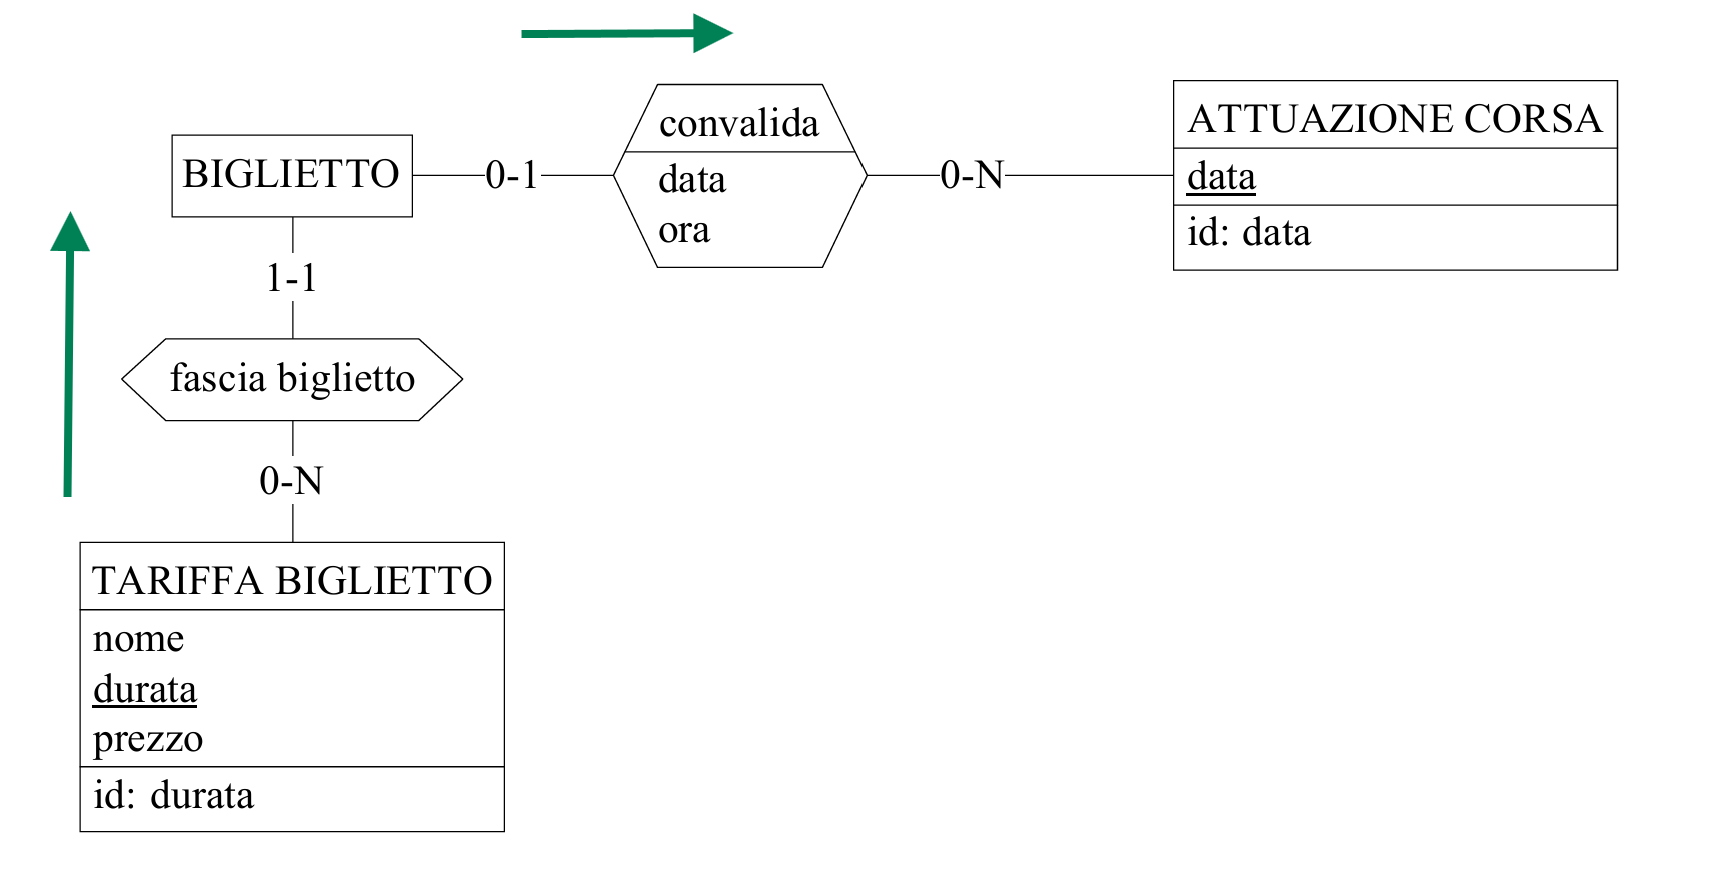
\includegraphics[width=0.7\textwidth]{VisualIncassoPerTariffa}
    \end{center}
    \begin{table}[H]
    \centering
    \begin{tabular}{|c|c|l|l|}
    \hline
    \textbf{Nome} & \textbf{Tipo} & \textbf{Numero accessi} & \textbf{S/L} \\
    \hline
    TARIFFA BIGLIETTO & E & 1 & L \\
    \hline
    BIGLIETTO & E & 30.000 & L \\
    \hline
    CONVALIDA & A & 20.000 & L \\
    \hline
    \multicolumn{4}{c}{\textbf{Totale}} \\    
    \multicolumn{4}{c}{${A_{lettura}}$ = 50.001, ${A_{scrittura}}$ = 0} \\
    \hline
    \end{tabular}
    \end{table}
    \begin{center}
    ${C_{tot} = {O_{settimana}}\cdot{A_{lettura}}= 250.005}$
    \end{center}

  % ------------------------------------------------------------------------------------------------------------------------------------------- 
  % ------------------------------------------------------------------------------------------------------------------------------------------- 

    \item\textbf{Estrazione delle linee con più multe negli ultimi 3 mesi} \label{op11} \\
	\[{O_{settimana} = 2}\]
	Questa operazione deve poter essere effettuata dall'amministratore di sistema.\\
	Per ogni linea va estratto:
	\begin{itemize}
	\renewcommand\labelitemi{--}
	    \item Il codice della linea
	    \item Il numero di multe ottenute negli ultimi 3 mesi
	\end{itemize}
	\begin{center}
	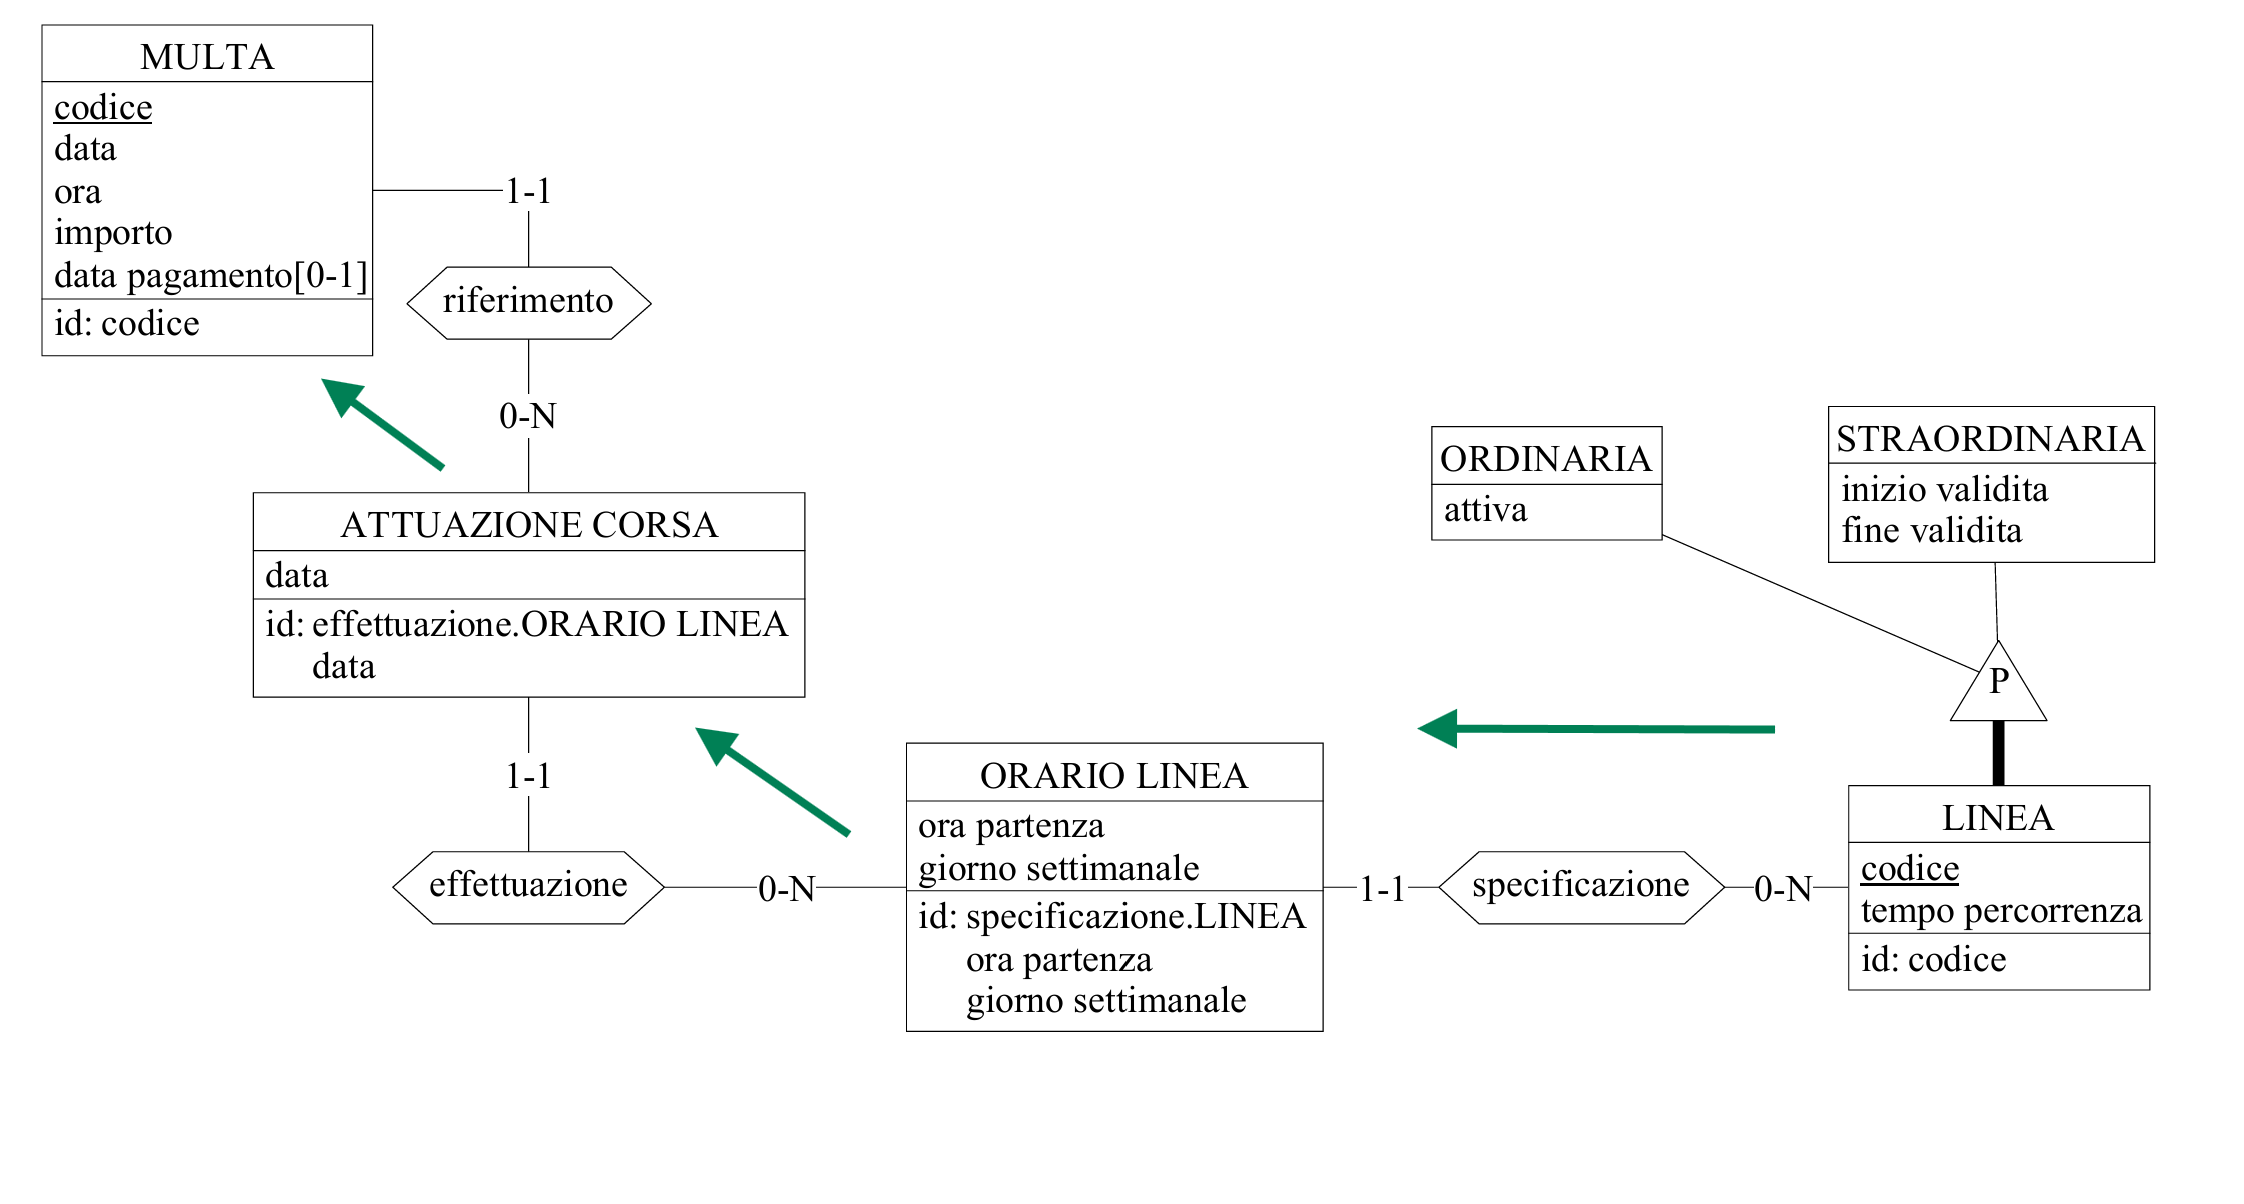
\includegraphics[width=0.7\textwidth]{VisualLineeConPiuMulte}
	\end{center}

	\begin{table}[H]
	\centering
	\begin{tabular}{|l|c|c|c|}
	\hline
	Nome & Tipo & Numero Accessi & S/L \\
	\hline
	LINEA & E & 75 & L \\
	\hline
	ORARIO LINEA & E & 75 $\times$ 20 & L \\
	\hline
	ATTUAZIONE CORSA & E & 3333 $\times$ 75 & L \\
	\hline
	MULTA & E & 0.04 $\times$ 75 & L \\
	    \hline
	    \multicolumn{4}{c}{\textbf{Totale}} \\    
	    \multicolumn{4}{c}{${A_{lettura}}$ = 251.850, ${A_{scrittura}}$ = 0} \\
	    \hline
	\end{tabular}
	\end{table}
	    \begin{center}
	    ${C_{tot} = {O_{settimana}}\cdot{A_{lettura}}= 503.700}$
	    \end{center}


  % ------------------------------------------------------------------------------------------------------------------------------------------- 
  % ------------------------------------------------------------------------------------------------------------------------------------------- 

	\item \textbf{Estrazione delle 5 linee con manutenzioni più gravose (in termini di linee sostitutive e durata)} \label{op12} \\
	    \[ {O_{settimana} = 2} \]
	    Dobbiamo visualizzare le linee con le manutenzioni più gravose, a livello applicativo verrà calcolato un "punteggio" che indicherà quanto sia gravosa una manutenzione:
	    \begin{itemize}
		\renewcommand\labelitemi{--}
	        \item +5 pti ogni linea straordinaria dovuta alla manutenzione
	        \item +1 pto ogni 3 giorni di lavoro sulla  linea.
	    \end{itemize}
        \begin{center}
	    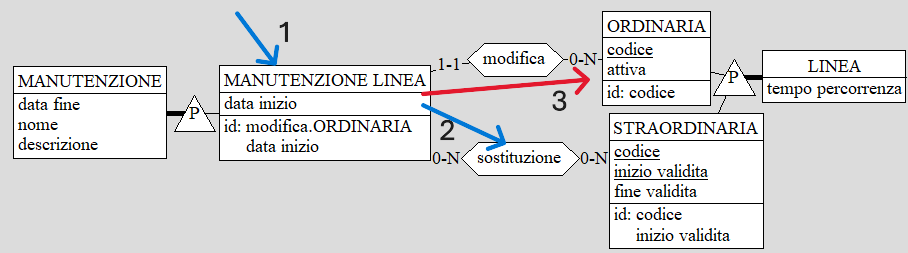
\includegraphics[width=0.9\textwidth]{op_12}
	    \end{center}
	    \begin{table}[H]
	    \centering
	    \begin{tabular}{|c|c|l|l|}
	    \hline
	    \textbf{Nome} & \textbf{Tipo} & \textbf{Numero accessi} & \textbf{S/L} \\
	    \hline
	    MANUTENZIONE LINEA & E & 10 & L \\ 
	    \hline
	    SOSTITUZIONE & A & 10 & L \\ 
	    \hline
	    LINEA ORDINARIA & E & 5 & L \\
	    \hline
	    \multicolumn{4}{c}{\textbf{Totale}} \\    
	    \multicolumn{4}{c}{${A_{lettura}}$ = 25, ${A_{scrittura}}$ = 0} \\
	    \hline
	    \end{tabular}
	    \end{table}
	    \begin{center}
	    ${C_{tot} = {O_{settimana}}\cdot {A_{lettura}} = 100}$
	    \end{center}

  % ------------------------------------------------------------------------------------------------------------------------------------------- 
  % ------------------------------------------------------------------------------------------------------------------------------------------- 
	\item \textbf{Estrazione delle linee con $>5$ controlli/giorno e $\leq 10$ multe/giorno} \label{op13} \\
	\[{O_{settimana} = 3}\]
	Questa operazione deve poter essere effettuata dall'amministratore di sistema.\\
	Devono essere estratti i codici delle linee che rispettano la seguente condizione:
	\[
	\text{controllo} > 5/\text{giorno} \cap \text{multe} \leq 10/\text{giorno}
	\]
	
	\begin{center}
	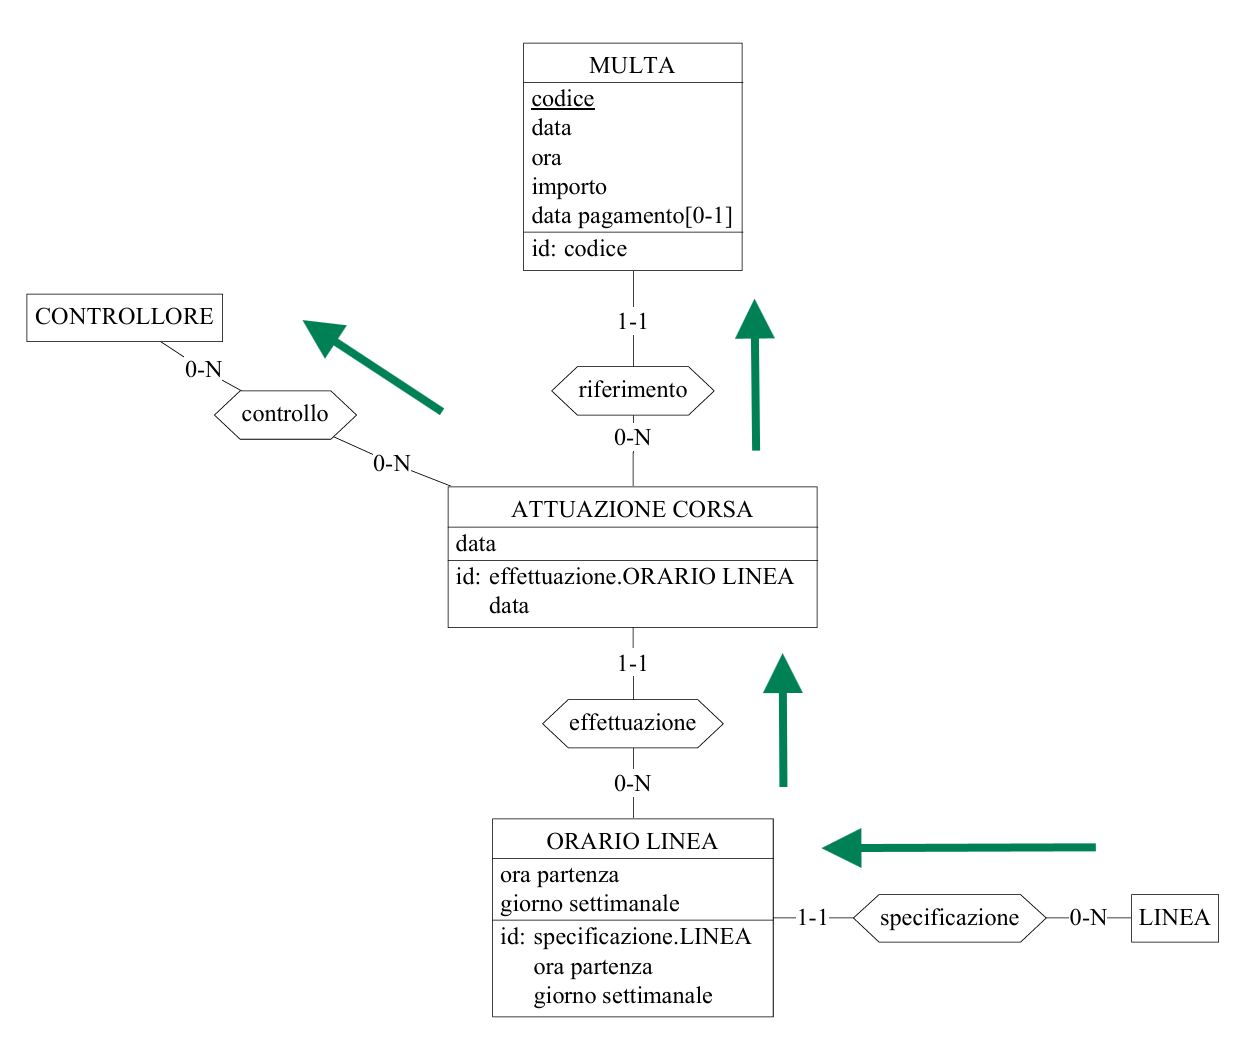
\includegraphics[width=0.7\textwidth]{VisualLineeMulteControlli}
	\end{center}
	
	\begin{table}[H]
	\centering
	\begin{tabular}{|l|c|c|c|}
	\hline
	Nome & Tipo & Numero Accessi & S/L \\
	\hline
	LINEA & E & 75 & L \\
	\hline
	ORARIO LINEA & E & 20 $\times$ 75 & L \\
	\hline
	ATTUAZIONE CORSA & E & 3333 $\times$ 75 & L \\
	\hline
	CONTROLLO & A & 0.2 $\times$ 75 & L \\
	    \hline
	    \multicolumn{4}{c}{\textbf{Totale}} \\    
	    \multicolumn{4}{c}{${A_{lettura}}$ = 251.700, ${A_{scrittura}}$ = 0} \\
	    \hline
	\end{tabular}
	\end{table}
	    \begin{center}
	    ${C_{tot} = {O_{settimana}}\cdot {A_{lettura}} = 755.100}$
	    \end{center}

  % ------------------------------------------------------------------------------------------------------------------------------------------- 
  % ------------------------------------------------------------------------------------------------------------------------------------------- 

    \item \textbf{Visualizzazione delle linee con il maggior tempo di percorrenza} \label{op14} \\
            \[ {O_{settimana} = 2} \]
           \begin{itemize}
            \item \textbf{Analisi con attributo ridondante \texttt{tempo percorrenza} su \texttt{LINEA}} \\
        In questo caso basterà leggere il dato del tempo di percorrenza dalla relativa linea.
        \begin{table}[H]
        \centering
        \begin{tabular}{|c|c|l|l|}
        \hline
        \textbf{Nome} & \textbf{Tipo} & \textbf{Numero accessi} & \textbf{S/L} \\
        \hline
        LINEA & E & 75 & L \\ 
        \hline
        \multicolumn{4}{c}{\textbf{Totale}} \\    
        \multicolumn{4}{c}{${A_{lettura}}$ = 75, ${A_{scrittura}}$ = 0} \\
        \hline
        \end{tabular}
        \end{table}
        \begin{center}
        ${C_{tot} = {O_{settimana}}\cdot {A_{lettura}} = 150}$
        \end{center}

            \item \textbf{Analisi senza attributo ridondante \texttt{tempo percorrenza} su \texttt{LINEA}} \\
        In questo caso invece dovremmo calcolare il tempo di percorrenza leggendo tutte le \texttt{tratte} di cui è composta la relativa linea.
        \begin{center}
	    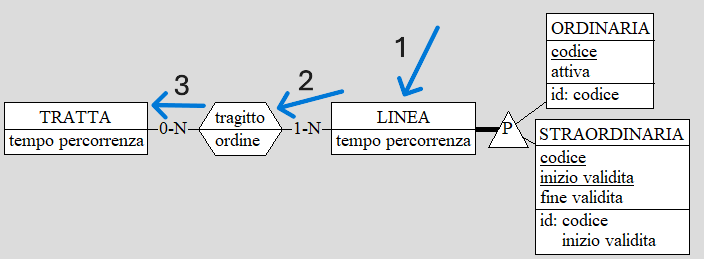
\includegraphics[width=0.7\textwidth]{op_14_NORID}
	    \end{center}
        \begin{table}[H]
        \centering
        \begin{tabular}{|c|c|l|l|}
        \hline
        \textbf{Nome} & \textbf{Tipo} & \textbf{Numero accessi} & \textbf{S/L} \\
        \hline
        LINEA & E & 75 & L \\ 
        \hline
        TRAGITTO & A & 1.500 & L \\
        \hline
        TRATTA & E & 1.500 & L \\
        \hline
        \multicolumn{4}{c}{\textbf{Totale}} \\    
        \multicolumn{4}{c}{${A_{lettura}}$ = 3.075, ${A_{scrittura}}$ = 0} \\
        \hline
        \end{tabular}
        \end{table}
        \begin{center}
        ${C_{tot} = {O_{settimana}}\cdot {A_{lettura}} = 6.150}$
        \end{center}     

	\end{itemize}

  % ------------------------------------------------------------------------------------------------------------------------------------------- 
  % ------------------------------------------------------------------------------------------------------------------------------------------- 
   
    \item\textbf{Estrazione delle linee con più hub mobilità lungo il percorso} \label{op15} \\
    \[ {O_{settimana} = 3} \]
    A fini statistici si vuole scoprire qual è la linea che contiene più Hub Mobilità, dati dalla somma di tutte gli Hub che stanno nelle varie fermate. \\
    Si vuole quindi estrarre:
    \begin{itemize}
	\renewcommand\labelitemi{--}
    \item Il codice della \texttt{LINEA} che contiene il maggior numero di hub
    \end{itemize}

    \begin{center}
    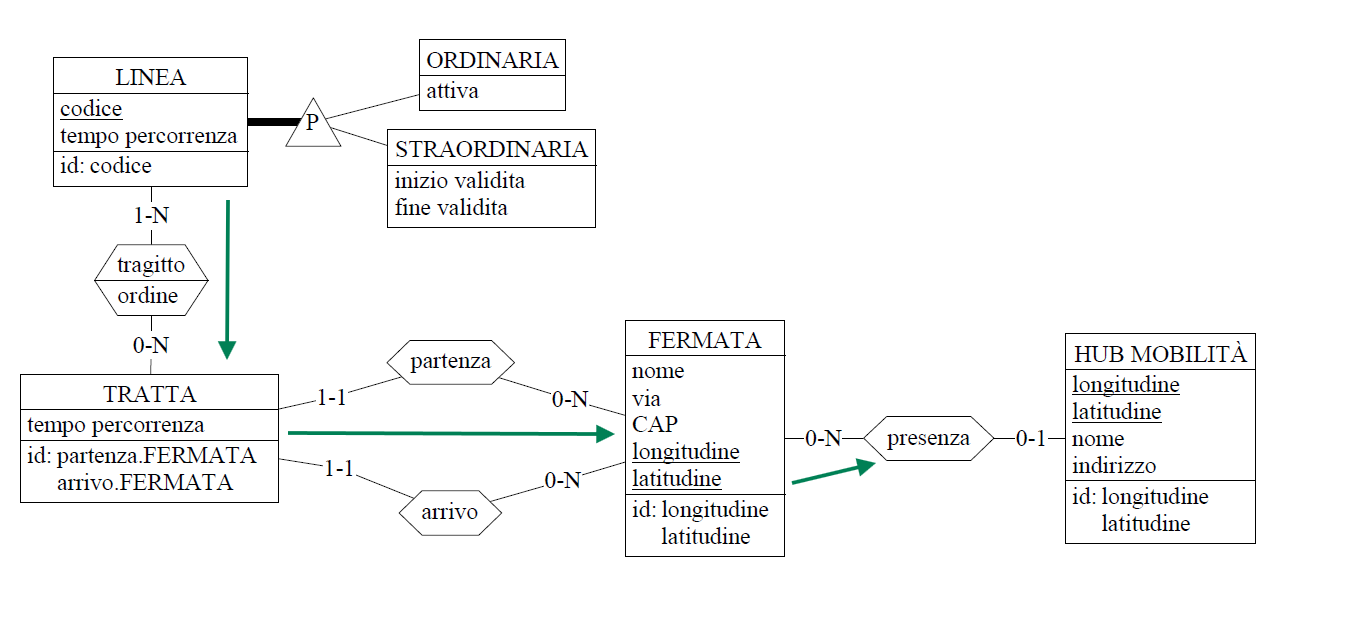
\includegraphics[width=0.9\textwidth]{VisualLineeMaggiorHub}
    \end{center}
    \begin{table}[H]
    \centering
    \begin{tabular}{|c|c|l|l|}
    \hline
    \textbf{Nome} & \textbf{Tipo} & \textbf{Numero accessi} & \textbf{S/L} \\
    \hline
    LINEA & E & 75 & L \\
    \hline
    TRAGITTO & A & 1.500 & L \\
    \hline
    TRATTA & E & 1.000 & L \\
    \hline
    FERMATA & E & 450 & L \\
    \hline
    PRESENZA & A & 165 & L \\
    \hline
    \multicolumn{4}{c}{\textbf{Totale}} \\    
    \multicolumn{4}{c}{${A_{lettura}}$ = 3.190, ${A_{scrittura}}$ = 0} \\
    \hline
    \end{tabular}
    \end{table}
    \begin{center}
    ${C_{tot} = {O_{settimana}}\cdot{A_{lettura}}= 9.570}$
    \end{center}

  % ------------------------------------------------------------------------------------------------------------------------------------------- 
  % ------------------------------------------------------------------------------------------------------------------------------------------- 

         \item\textbf{Media di soldi spesi in multe per persona} \label{op16} \\
	\[{O_{settimana} = 1}\]
	Questa operazione deve poter essere effettuata dall'amministratore di sistema.\\
	Deve essere estratto un unico numero, ovvero la media del prezzo totale pagato per persona.	
	\begin{table}[H]
	\centering
	\begin{tabular}{|l|c|c|c|}
	\hline
	Nome & Tipo & Numero Accessi & S/L \\
	\hline
	MULTA & E & 10000 & L \\
	\hline
	CAUSALE MULTA & E & 10000 & L \\
	    \hline
	    \multicolumn{4}{c}{\textbf{Totale}} \\    
	    \multicolumn{4}{c}{${A_{lettura}}$ = 20.000, ${A_{scrittura}}$ = 0} \\
	    \hline
	    \end{tabular}
	    \end{table}
	    \begin{center}
	    ${C_{tot} = {O_{settimana}}\cdot{A_{lettura}}= 20.000}$
	    \end{center}

  % ------------------------------------------------------------------------------------------------------------------------------------------- 
  % ------------------------------------------------------------------------------------------------------------------------------------------- 

	\item \textbf{Visualizzazione delle aziende che non hanno effettuato nessuna manutenzione nell’ultimo mese} \label{op17} \\
    \[ {O_{settimana} = 4} \]
    \begin{center}
	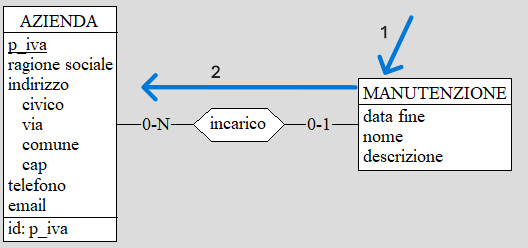
\includegraphics[width=0.7\textwidth]{op_17}
	\end{center}
    \begin{table}[H]
    \centering
    \begin{tabular}{|c|c|l|l|}
    \hline
    \textbf{Nome} & \textbf{Tipo} & \textbf{Numero accessi} & \textbf{S/L} \\
    \hline
    MANUTENZIONE & E & 50 & L \\ 
    \hline
    AZIENDA & E & x & L \\ 
    \hline
    \multicolumn{4}{c}{\textbf{Totale}} \\    
    \multicolumn{4}{c}{${A_{lettura}}$ = 50 + x, ${A_{scrittura}}$ = 0} \\
    \hline
    \end{tabular}
    \end{table}
    \begin{center}
    ${C_{tot} = {O_{settimana}}\cdot {A_{lettura}} = 200 + 4x}$
    \end{center}

  % ------------------------------------------------------------------------------------------------------------------------------------------- 
  % ------------------------------------------------------------------------------------------------------------------------------------------- 

    \item\textbf{Visualizzazione delle fermate in cui è presente almeno un hub mobilità contenente tutti i tipi di servizi green} \label{op18} \\
    \[ {O_{settimana} = 1} \]
    Questa operazione punta a ricercare le fermate più eco-friendly, ovvero che fanno riferimento ad almeno un hub mobilità che contenga TUTTI i tipi di servizi possibili. Si tratta quindi di un'operazione di divisione. \\    
    Si vuole quindi visualizzare:
    \begin{itemize}
	\renewcommand\labelitemi{--}
    \item L'elenco dei nomi di tutte le \texttt{FERMATA} che rispettano le specifiche
    \end{itemize}
    \begin{center}
    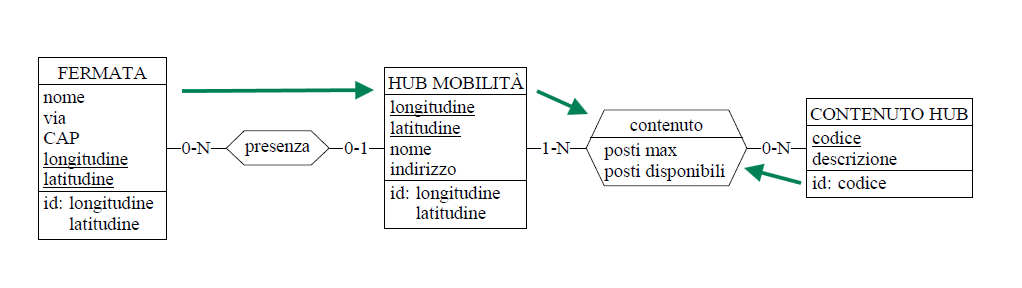
\includegraphics[width=0.8\textwidth]{VisualFermateHubCompleti}
    \end{center}
    \begin{table}[H]
    \centering
    \begin{tabular}{|c|c|l|l|}
    \hline
    \textbf{Nome} & \textbf{Tipo} & \textbf{Numero accessi} & \textbf{S/L} \\
    \hline
    FERMATA & E & 450 & L \\
    \hline
    HUB MOBILITA & E & 225 & L \\
    \hline
    CONTENUTO & A & 450 & L \\
    \hline
    CONTENUTO HUB & E & 4 & L \\
    \hline
    \multicolumn{4}{c}{\textbf{Totale}} \\    
    \multicolumn{4}{c}{${A_{lettura}}$ = 1.129, ${A_{scrittura}}$ = 0} \\
    \hline
    \end{tabular}
    \end{table}
    \begin{center}
    ${C_{tot} = {O_{settimana}}\cdot{A_{lettura}}= 1.129}$
    \end{center}


  % ------------------------------------------------------------------------------------------------------------------------------------------- 
  % ------------------------------------------------------------------------------------------------------------------------------------------- 
    \item\textbf{Inserimento di una variazione di servizio} \label{op19} \\
	\[{O_{settimana} = 1}\]
	Questa operazione deve poter essere effettuata dall'amministratore di sistema.\\
	Supponendo che le linee straordinarie sostitutive siano già state inserite, si deve creare una nuova manuntenzione.\\
	Alla manuntenzione va indicata la linea che viene modificata, e le eventuali linee che la sostituiscono.\\
	Inoltre se l'inizio della manuntenzione è immediato, allora la linea coinvolta va disattivata.\\
	\textbf{OSS: va calcolato l'impatto di avere o no l'attributo ridondante \texttt{ATTIVA}}
          
	 \begin{itemize}
            \item \textbf{Analisi con attributo ridondante \texttt{attiva} su \texttt{LINEA}} \\
	\begin{center}
	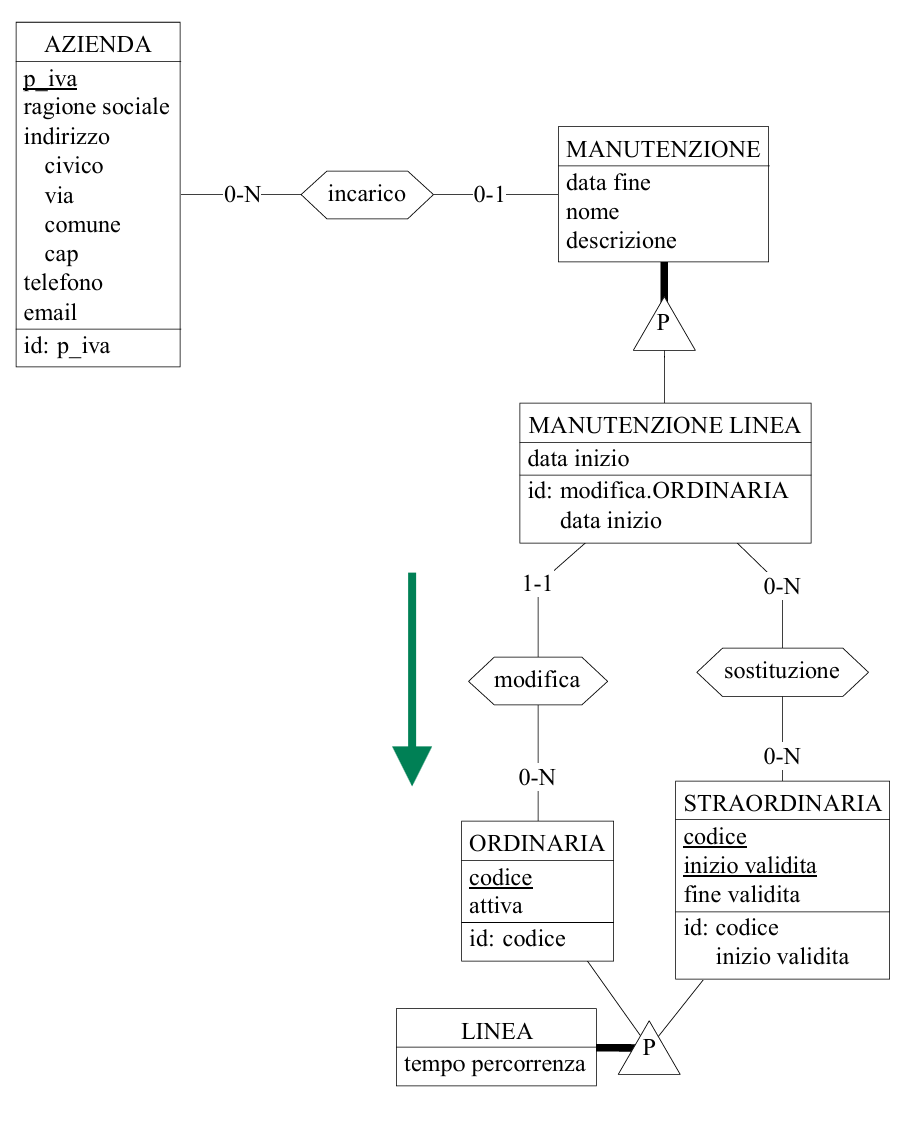
\includegraphics[width=0.6\textwidth]{InserimentoVariazioneServizioRid}
	\end{center}
	\begin{table}[H]
	\centering
	\begin{tabular}{|l|c|c|c|}
	\hline
	Nome & Tipo & Numero Accessi & S/L \\
	\hline
	MANUNTENZIONE LINEA & E & 1 & S \\
	\hline
	ORDINARIA & E & 1 & L \\
	\hline
	ORDINARIA & E & 1 & S \\
	\hline
	SOSTITUZIONE & A & 1 & S \\
	\hline
	    \multicolumn{4}{c}{\textbf{Totale}} \\    
	    \multicolumn{4}{c}{${A_{lettura}}$ = 1, ${A_{scrittura}}$ = 3} \\
	    \hline
	    \end{tabular}
	    \end{table}
	    \begin{center}
	    ${C_{tot} = {O_{settimana}}\cdot({A_{lettura}} + {2A_{scrittura}})= 7}$
	    \end{center}

            \item \textbf{Analisi senza attributo ridondante \texttt{attiva} su \texttt{LINEA}} \\
	\begin{center}
	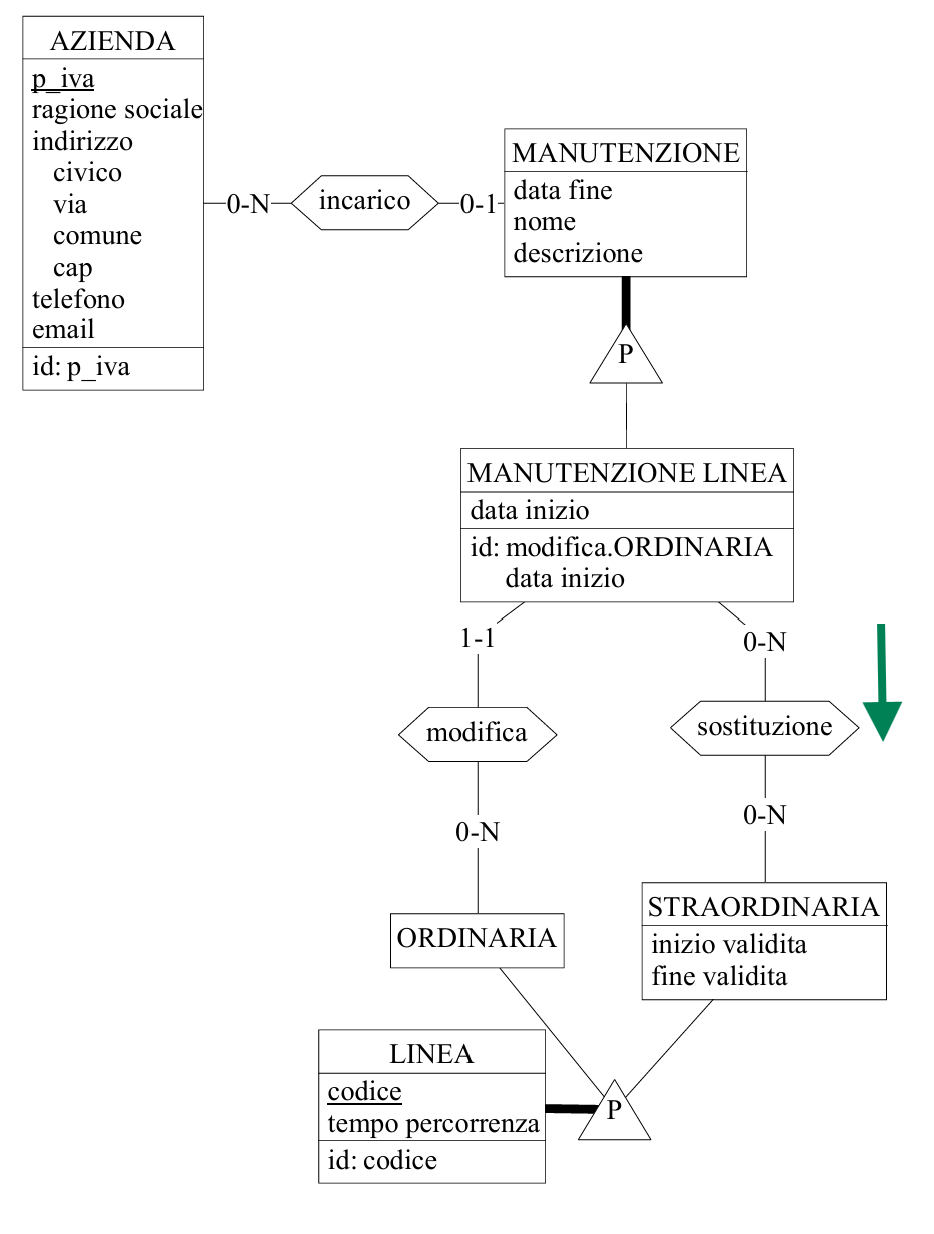
\includegraphics[width=0.8\textwidth]{InserimentoVariazioneServizioNoRid}
	\end{center}
	\begin{table}[H]
	\centering
	\begin{tabular}{|l|c|c|c|}
	\hline
	Nome & Tipo & Numero Accessi & S/L \\
	\hline
	MANUNTENZIONE LINEA & E & 1 & S \\
	\hline
	SOSTITUZIONE & A & 1 & S \\
	\hline
	    \multicolumn{4}{c}{\textbf{Totale}} \\    
	    \multicolumn{4}{c}{${A_{lettura}}$ = 0, ${A_{scrittura}}$ = 2} \\
	    \hline
	    \end{tabular}
	    \end{table}
	    \begin{center}
	    ${C_{tot} = {O_{settimana}}\cdot({A_{lettura}} + {2A_{scrittura}})= 4}$
	    \end{center}
	
	\end{itemize}
	

  % ------------------------------------------------------------------------------------------------------------------------------------------- 
  % ------------------------------------------------------------------------------------------------------------------------------------------- 

    \item\textbf{Aggiunta di una tratta a una linea esistente} \label{op20} \\
    \[ {O_{settimana} = 1} \]
    Questa operazione serve per aggiornare una linea, aggiungendo una fermata al suo tragitto. Nell'analisi terremo conto che la fermata va aggiunta dopo il capolinea, ovvero è necessario solo aggiungere la tratta per poi aggiungerla al traggito. Visto che il tempo di percorrenza di una linea è calcolabile anche come la somma dei tempi di percorrenza delle tratte, si rende necessaria l'analisi differenziata per la presenza dell'attributo \texttt{tempo percorrenza} su \texttt{LINEA}, poiché in caso di ridondanza sarà necessario rieseguire il calcolo del tempo totale per poi aggiornare l'attributo.
    
    \begin{itemize}
    \item \textbf{Analisi con attributo ridondante \texttt{tempo percorrenza} su \texttt{LINEA}}
    \begin{center}
    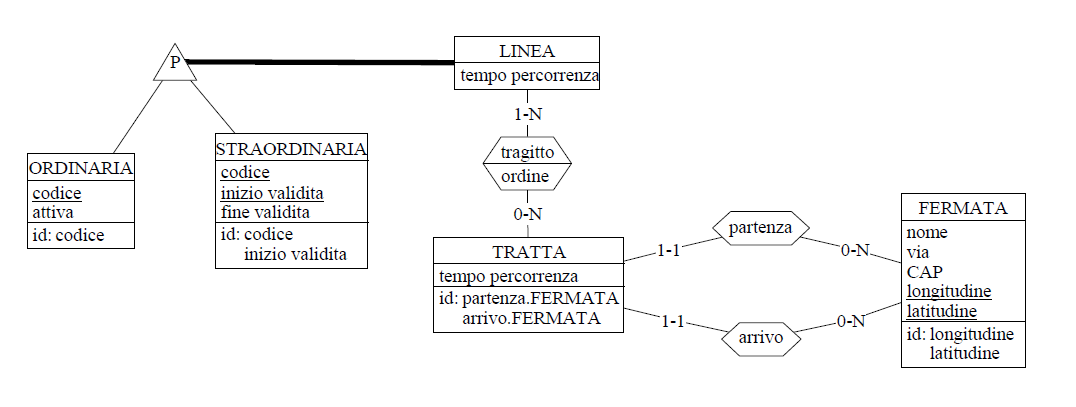
\includegraphics[width=0.8\textwidth]{AggiornaLineaRid}
    \end{center}
    \begin{table}[H]
    \centering
    \begin{tabular}{|c|c|l|l|}
    \hline
    \textbf{Nome} & \textbf{Tipo} & \textbf{Numero accessi} & \textbf{S/L} \\
    \hline
    TRATTA & E & 1 & S \\
    \hline
    TRAGITTO & A & 1 & S \\
    \hline
    TRATTA & A & 21 & L \\
    \hline
    LINEA & E & 1 & S + L \\
    \hline
    \multicolumn{4}{c}{\textbf{Totale}} \\    
    \multicolumn{4}{c}{${A_{lettura}}$ = 22, ${A_{scrittura}}$ = 3} \\
    \hline
    \end{tabular}
    \end{table}
    \begin{center}
    ${C_{tot} = {O_{settimana}}\cdot({A_{lettura}} + {2A_{scritttura}})= 28}$
    \end{center}
    \item \textbf{Analisi senza attributo ridondante \texttt{tempo percorrenza} su \texttt{LINEA}}
    \begin{center}
    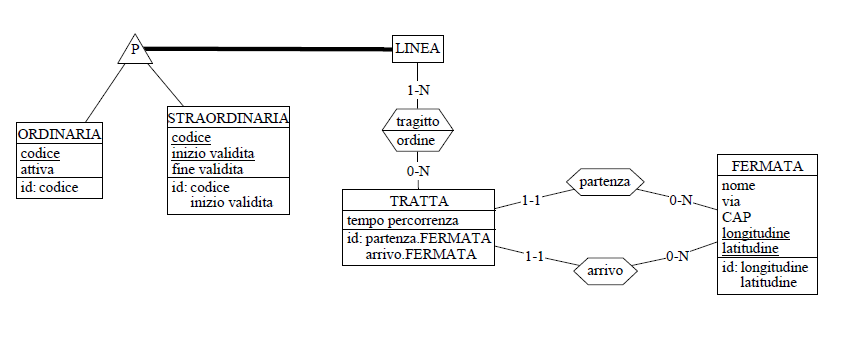
\includegraphics[width=0.8\textwidth]{AggiornaLineaNoRid}
    \end{center}
    \begin{table}[H]
    \centering
    \begin{tabular}{|c|c|l|l|}
    \hline
    \textbf{Nome} & \textbf{Tipo} & \textbf{Numero accessi} & \textbf{S/L} \\
    \hline
    TRATTA & E & 1 & S \\
    \hline
    TRAGITTO & A & 1 & S \\
    \hline
    \multicolumn{4}{c}{\textbf{Totale}} \\    
    \multicolumn{4}{c}{${A_{lettura}}$ = 0, ${A_{scrittura}}$ = 2} \\
    \hline
    \end{tabular}
    \end{table}
    \begin{center}
    ${C_{tot} = {O_{settimana}}\cdot{2A_{scritttura}}= 4}$
    \end{center}
    \end{itemize}


  % ------------------------------------------------------------------------------------------------------------------------------------------- 
  % ------------------------------------------------------------------------------------------------------------------------------------------- 

    \item\textbf{Creazione di una nuova linea} \label{op21} \\
	\[{O_{settimana} = 1}\]
	Questa operazione deve poter essere fatta dall'amministratore di sistema.\\
	Supponendo che le tratte siano già definite, per ogni linea va indicato l'insieme delle tratte che percorre e, per ogni tratta, specificare l'ordine con cui viene percorsa.\\
	Inoltre vanno sommati i tempi di percorrenza di ogni tratta per calcolare il campo \texttt{tempo percorrenza}

	 \begin{itemize}
    	\item \textbf{Analisi con attributo ridondante \texttt{tempo percorrenza} su \texttt{LINEA}}
	\begin{center}
	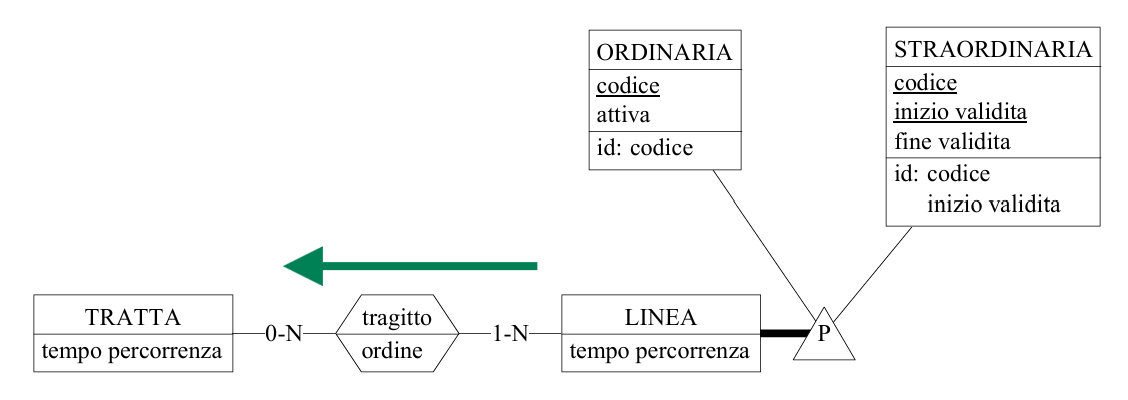
\includegraphics[width=0.7\textwidth]{InserimentoLineaRid}
	\end{center}
	\begin{table}[H]
	\centering
	\begin{tabular}{|l|c|c|c|}
	\hline
	Nome & Tipo & Numero Accessi & S/L \\
	\hline
	LINEA & E & 1 & S \\
	\hline
	TRAGITTO & A & 20 & S \\
	\hline
	TRATTA & E & 20 & L \\
	\hline
	    \multicolumn{4}{c}{\textbf{Totale}} \\    
	    \multicolumn{4}{c}{${A_{lettura}}$ = 21, ${A_{scrittura}}$ = 20} \\
	    \hline
	    \end{tabular}
	    \end{table}
	    \begin{center}
	    ${C_{tot} = {O_{settimana}}\cdot{2A_{scritttura}}= 61}$
	    \end{center}

	\item \textbf{Analisi con attributo ridondante \texttt{tempo percorrenza} su \texttt{LINEA}}
	\begin{center}
	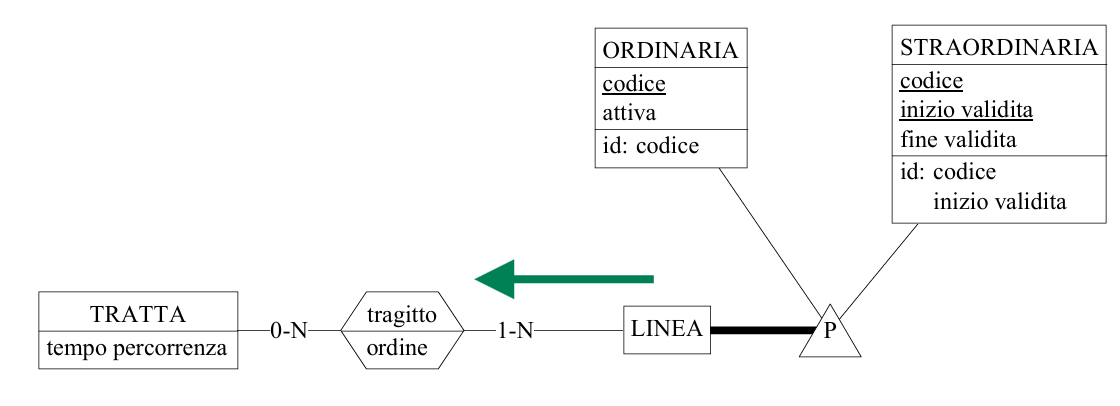
\includegraphics[width=0.7\textwidth]{InserimentoLineaNoRid}
	\end{center}
	\begin{table}[H]
	\centering
	\begin{tabular}{|l|c|c|c|}
	\hline
	Nome & Tipo & Numero Accessi & S/L \\
	\hline
	LINEA & E & 1 & S \\
	\hline
	TRAGITTO & A & 20 & S \\
	\hline
	    \multicolumn{4}{c}{\textbf{Totale}} \\    
	    \multicolumn{4}{c}{${A_{lettura}}$ = 1, ${A_{scrittura}}$ = 20} \\
	    \hline
	    \end{tabular}
	    \end{table}
	    \begin{center}
	    ${C_{tot} = {O_{settimana}}\cdot{2A_{scritttura}}= 41}$
	    \end{center}
	\end{itemize}
\end{enumerate}

\section{Analisi delle ridondanze}
In questa sezione andremo ad analizzare le due ridondanze presenti nel modello, ovvero:
\begin{itemize}
  \item \texttt{tempo percorrenza} su \texttt{LINEA}
  \item \texttt{attiva} su \texttt{LINEA}
\end{itemize}

\subsection{Analisi attributo \texttt{tempo percorrenza}}

\begin{table}[H]
	\centering
	\begin{tabular}{|l|c|c|c|}
	\hline
	\textbf{Num Op.} & \textbf{Con ridondanza} & \textbf{Senza ridondanza} \\
	\hline
	4 & 1.153.950 & 12.691.950 \\
  \hline
	5 & 252.200 & 280.200 \\
  \hline
  14 & 150 & 6.150 \\
  \hline
  20 & 28 & 4 \\
  \hline
  21 & 61 & 41 \\
  \hline
  \textbf{TOTALE} & \textbf{1.406.389} & \textbf{12.978.345} \\
  \hline
  \end{tabular}
\end{table}

A fronte di questa analisi, decidiamo di mantenere l'attributo \texttt{tempo percorrenza}.

\subsection{Analisi attributo \texttt{attiva}}

  \begin{table}[H]
  \centering
  \begin{tabular}{|l|c|c|c|}
  \hline
  \textbf{Num Op.} & \textbf{Con ridondanza} & \textbf{Senza ridondanza} \\
  \hline
  1 & 1.950 & 7.800.000 \\
  \hline
  19 & 7 & 4 \\
  \hline
  \textbf{TOTALE} & \textbf{1.957} & \textbf{7.800.004} \\
  \hline
  \end{tabular}
\end{table}

A fronte di questa analisi, decidiamo di mantenere l'attributo \texttt{attiva}.

\section{Riepilogo operazioni}
Nella seguente tabella proponiamo un riepilogo delle operazioni analizzate, con il costo totale per ogni operazione.

\begin{longtable}{|c|p{8cm}|c|l|l|}
\caption{Costo totale delle operazioni stimato per 7 giorni}
\label{table:operazioni_tot}\\
\hline
\textbf{\#} & \textbf{Operazione} & \textbf{Costo tot. / 7gg} & \textbf{Tipo Utente} \\
\hline
\endhead
1  & \hyperref[op1]{Visualizzazione di tutte le linee attive} & 7.800.000 & Tutti \\
\hline
2 & \hyperref[op2]{Visualizzazione fermate e orari di una linea} & 248.500 & Tutti \\
\hline
3 & \hyperref[op3]{Visualizzazione degli hub mobilità} & 645.000 & Tutti \\
\hline
4* & \hyperref[op4]{Visualizzazione orario e mezzo assegnato} & 1.153.950 & Autista \\
\hline
5* & \hyperref[op5]{Visualizzazione orario e linee assegnate} & 252.200 & Controllore \\
\hline
6 & \hyperref[op6]{Estrazione delle linee con più convalide nell'ultimo mese} & 850.005 & Amministratore  \\
\hline
7 & \hyperref[op7]{Estrazione delle manuntenzioni che coinvolgono un determinato mezzo} & 35 & Amministratore \\
\hline
8 & \hyperref[op8]{Estrazione delle manuntenzioni ed eventuali linee sostitutive che coinvolgono una linea} & 205 & Amministratore \\
\hline
9 & \hyperref[op9]{Visualizzazione incassi dati dalle convalide per una linea} & 8.150 & Amministratore \\
\hline
10 & \hyperref[op10]{Estrazione degli incassi per tipo di titolo in periodo definito} & 250.005 & Amministratore \\
\hline
11 & \hyperref[op11]{Estrazione delle linee con più multe negli ultimi 3 mesi} & 503.700 & Amministratore \\
\hline
12 & \hyperref[op12]{Estrazione delle 5 linee con manutenzioni più gravose (in termini linee sostitutive e durata)} & 100 & Amministratore  \\
\hline
13 & \hyperref[op13]{Estrazione delle linee con \textgreater 5 controlli/giorno e \textless = 10 multe/giorno} & 755.100 & Amministratore  \\
\hline
14* & \hyperref[op14]{Visualizzazione delle linee con il maggior tempo di percorrenza} & 150 & Amministratore  \\
\hline
15 & \hyperref[op15]{Estrazione delle linee con più hub mobilità lungo il percorso} & 9.570 & Amministratore \\
\hline
16 & \hyperref[op16]{Media di soldi spesi in multe per persona} & 20.000 & Amministratore \\
\hline
17 & \hyperref[op17]{Visualizzazione delle aziende che non hanno effettuato nessuna manutenzione nell'ultimo mese} & 4XXX & Amministratore \\
\hline
18 & \hyperref[op18]{Visualizzazione delle fermate in cui è presente un hub mobilità contenente tutti i tipi di servizi green} & 1.129 & Amministratore \\
\hline
19* & \hyperref[op19]{Inserimento di una variazione di servizio} & 7 & Amministratore \\
\hline
20* & \hyperref[op20]{Aggiunta di una tratta a una linea esistente} & 28 & Amministratore \\
\hline
21* & \hyperref[op21]{Creazione di una nuova linea} & 61 & Amministratore \\
\hline
\end{longtable}

\section{Raffinamento dello schema}
Ora che abbiamo deciso quali attributi dovranno rimanere nella base di dati, non ci resta che apportare dei raffinamenti allo schema ER in modo da rielaborare i concetti non direttamente rappresentabili tramite il modello relazionale.
Procediamo quindi per step successivi fino ad arrivare a uno schema logico equivalente allo schema ER.

\subsection{Rimozione attributi multivalore}
L'unico attributo multivalore nel nostro schema è presente nell'entità \texttt{AZIENDA}, nello specifico l'\texttt{indirizzo}.
Aggiungiamo quindi il prefisso \texttt{indirizzo\textunderscore} a ogni suo componente per poi decomporlo in attributi singoli.

\subsection{Rimozione gerarchie}

\subsubsection{Biglietto}
La gerarchia su biglietto è di tipo Totale ed Esclusiva.
Poiché non ci sono attributi diversi nelle due entità figlie e \texttt{BIGLIETTO DIGITALE} ha l'associazione \texttt{acquisto} di cardinalità (1,1), scegliamo di effettuare un \textbf{collasso vero l'alto}. 
L'associazione \texttt{aquisto} diventa quindi a cardinalità (0, 1). \\
Sarà possibile riconoscere i biglietti digitali dai fisici perché questi ultimi non avranno l'associazione \texttt{acquisto} con l'entità \texttt{UTENTE}.

\subsubsection{Titolo di Viaggio}
Anche in questo caso la gerarchia è di tipo Totale ed Esclusiva.
Dal momento che le entità figlie hanno associazioni e attributi diversi, scegliamo di effettuare un \textbf{collasso vero il basso} che ci permette di mantenere questi vincoli inalterati.

\begin{figure}[H]
	\centering
	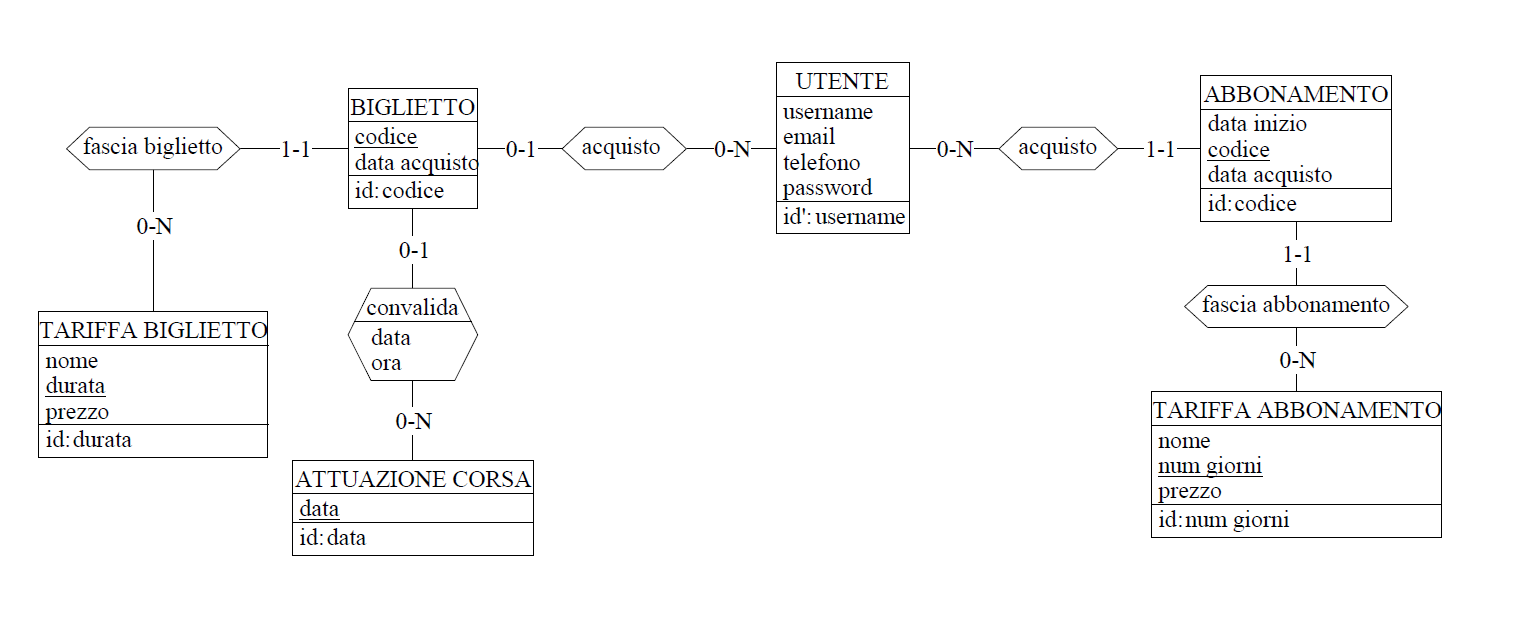
\includegraphics[width=1\textwidth]{GerarchiaTitoloViaggio}
 	\caption{Entità Biglietto e Abbonamento dopo la rimozione delle gerarchie}
\end{figure}

\subsubsection{Persona - Utente}
Abbiamo che \texttt{UTENTE} è un subset di \texttt{PERSONA}.
Se venisse effettuato un collasso avremmo vari attributi opzionali da gestire: scegliamo quindi di sostituire la gerarchia con un'\textbf{associazione}.
Così facendo a una persona fisica può essere connessa un'utenza, e a un'utenza deve per forza essere connessa una persona.

\subsubsection{Utente - Dipendente}
Come per Persona e Utente il subset è stato sostituito dall'associazione \texttt{dipendenza}, visto che le entità \texttt{UTENTE} e \texttt{DIPENDENTE} hanno associazioni diverse.

\subsubsection{Dipendente}
La gerarchia sui vari tipi di dipendente (\texttt{AMMINISTRATIVO}, \texttt{AUTISTA}, \texttt{CONTROLLORE}) è di tipo Totale ed Esclusiva.
Visto che le sottoentità non hanno attributi diversificati, scegliamo di fare un \textbf{collasso verso l'alto}.
Introduciamo un selettore di tipo chiamato \texttt{ruolo} che potrà assumere solo i valori di Amministrativo, Autista o Controllore. 
Visto che le associazioni specifiche per ogni ruolo ora fanno riferimento al generico dipendente sarà necessario porre attenzione ad eseguire dei controlli per verificare che si possano aggiungere delle associazioni solo se coerenti con il ruolo del dipendente coinvolto.

\begin{figure}[H]
	\centering
	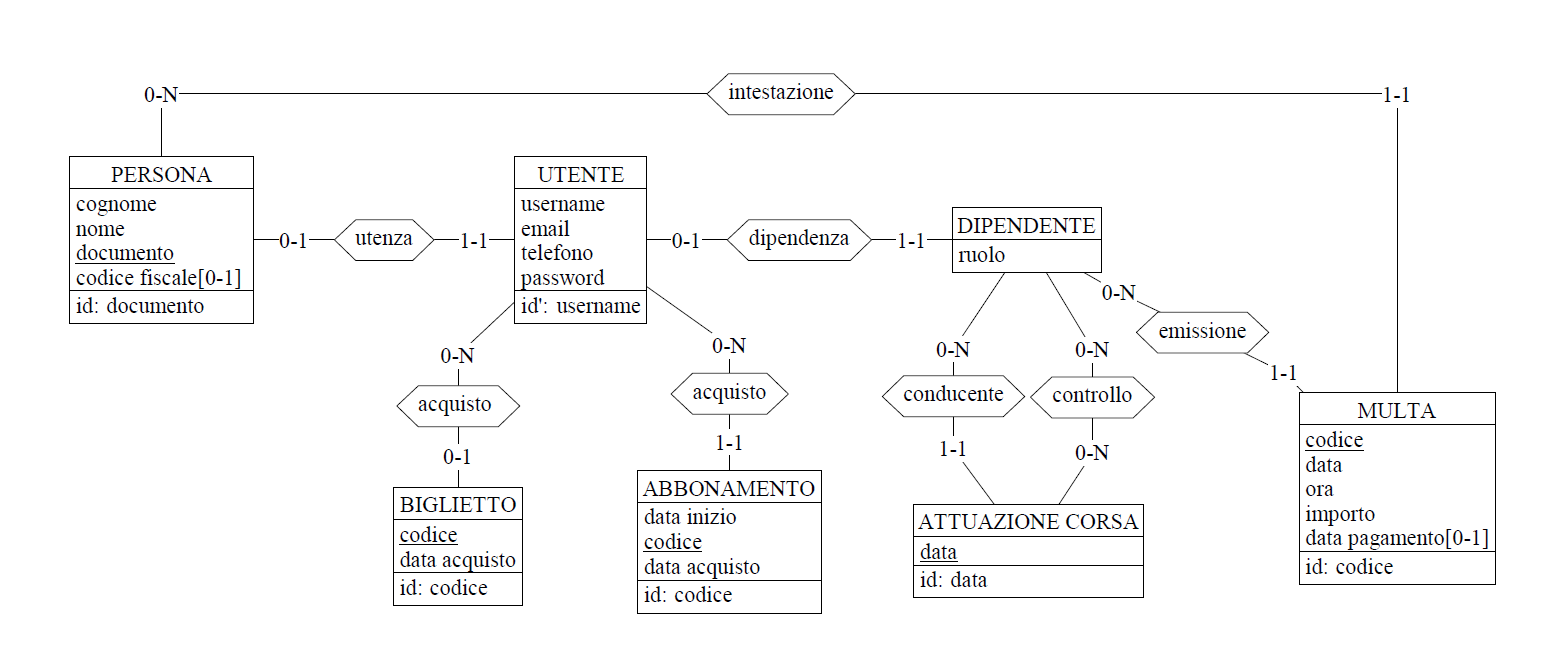
\includegraphics[width=1\textwidth]{GerarchiaPersona}
 	\caption{Entità Persona, Utente e Dipendente dopo la rimozione delle gerarchie}
\end{figure}

\subsubsection{Manutenzione}
La gerarchia su \texttt{MANUTENZIONE} è di tipo Totale ed Esclusiva.
Poiché le due entità figlie si riferiscono a due concetti differenti, quindi hanno anche associazioni diverse, scegliamo di effettuare un \textbf{collasso verso il basso} per mantenere i vincoli sulle associazioni. 
Importiamo quindi sui due figli gli attributi comuni e l'associazione comune \texttt{incarico}.

\subsubsection{Linea}
Le linee di tipo ordinario e straordinario compongono una gerarchia Totale ed Esclusiva.
Scegliamo di eseguire un \textbf{collasso verso l'alto}, così da avere tutte le linee in un'unica entità visto che sono oggetto di molte richieste comuni.
Dal momento che hanno alcuni attributi diversi, questi diventeranno degli opzionali e ci serviranno per capire di che tipo è la linea.

\begin{figure}[H]
	\centering
	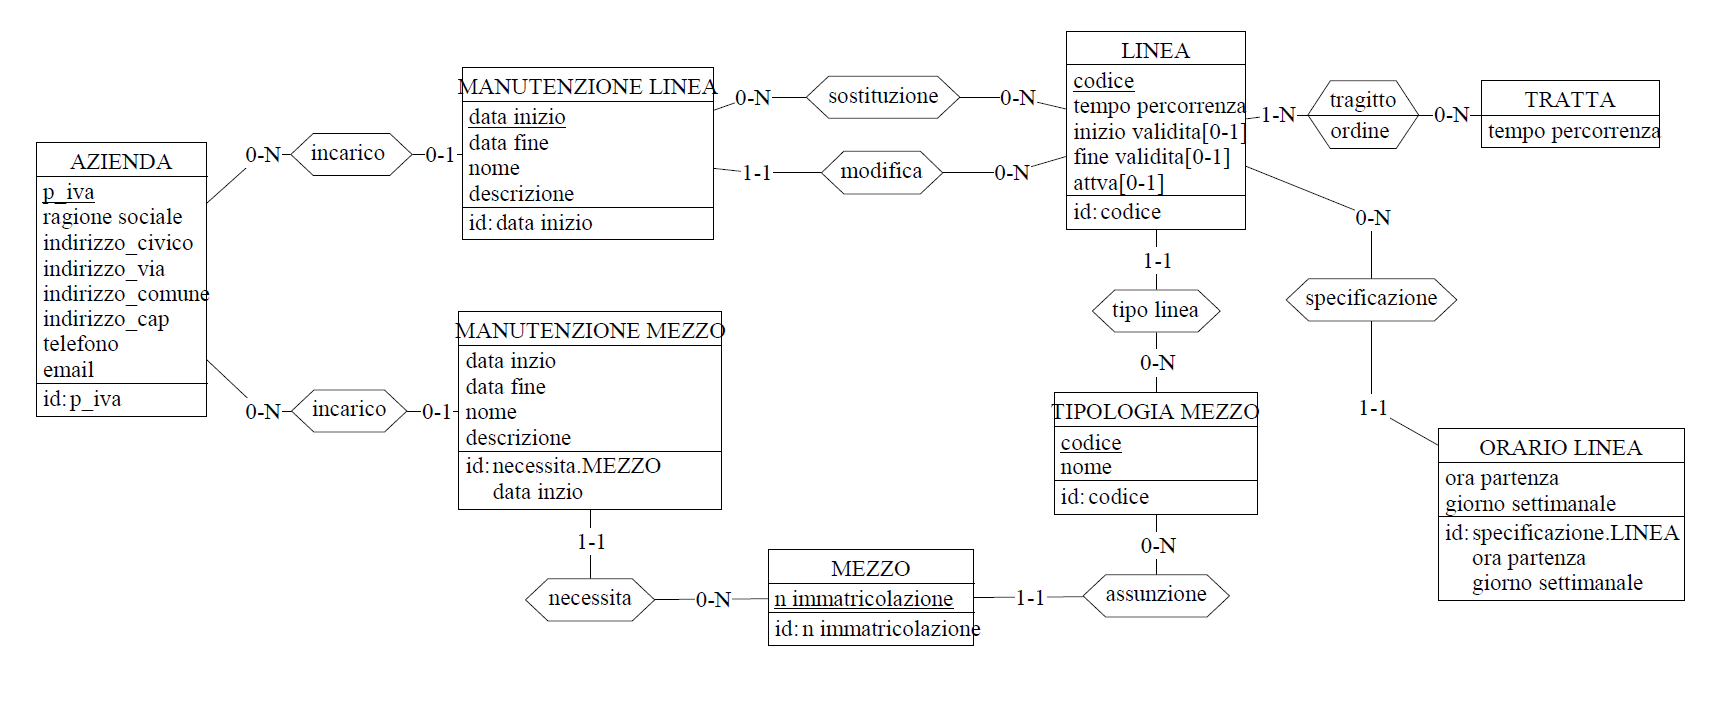
\includegraphics[width=1\textwidth]{GerarchiaLineaManutenzione}
 	\caption{Entità Manutenzione e Linea dopo la rimozione delle gerarchie}
\end{figure}

\subsection{Reificazione associazioni molti a molti}
Le associazioni \texttt{N-N} non sono direttamente rappresentabili nei database relazionali, quindi per ovviare a questo problema, le associazioni subiscono un processo di \textbf{reificazione} che comporta la trasformazione dell'associazione \texttt{N-N} in un'entità che sarà connessa con due associazioni \texttt{1-1} alle entità che prima collegava.\\ \\
Qui elencate troviamo le associazioni che sono state reificate:
\begin{itemize}
    \item Contenuto
    \item Tragitto
    \item Sostituzione
    \item Controllo
\end{itemize}

\subsection{Scelta degli identificatori principali}
Tutte le entità del nostro dominio sono già dotate dei loro identificatori principali naturali.
Per comodità ne sostituiamo alcuni con un semplice codice (lasciando comunque il vincolo di unicità su quelli esistenti) per rendere più semplici le query.\\
Riportiamo l'elenco delle entità in cui è stata effettuata quest'aggiunta:
\begin{itemize}
    \item Fermata
    \item Hub mobilità
    \item Orario linea
    \item Causale multa
    \item Attuazione Corsa
\end{itemize}

\section{Schema relazionale finale}
A questo punto tutti i problemi sono stati risolti, e il nostro schema ristrutturato è direttamente traducibile in delle relazioni.
\chapter{Progettazione dell'Applicazione}
\end{document}